\documentclass[12pt, a4paper]{article}
\usepackage{amsmath} % Required for inserting some mathematical notations and commands
\usepackage{hyperref} % Required for inserting hyperlinks
\usepackage{graphicx} % Required for inserting images
\usepackage{geometry} % Setting margins
\usepackage{lipsum} % Sample text generation
\usepackage{afterpage} % Required for \myemptypage
\usepackage{setspace} % Required for setting line spacing
\usepackage{booktabs} % Required for tables
\usepackage{multirow} % Required for the summary table's frame grouping
\usepackage{tikz} % Required for the methodology schematics
\usetikzlibrary{arrows.meta, positioning, fit, backgrounds, calc, decorations.pathreplacing}
\usepackage{float} % Required for figure placement control
\usepackage{caption} % Required for figure captions
\usepackage{subcaption} % Required for multi-panel figures
\usepackage[backend=biber, style=numeric, natbib=true, sorting=none]{biblatex} % Required for bibliography
\addbibresource{ref.bib} % Adds the bibliography reference
\graphicspath{{figs/}}
\raggedbottom

\begin{document}
% ---------------------------------------------------------------------------
% utilities.tex -- shared macros and page setup
% ---------------------------------------------------------------------------

% utilities.tex is \include-d AFTER \begin{document}, so preamble-only commands
% (\geometry, \usepackage, ...) cannot be used here. \newgeometry is the in-body form.
\newgeometry{margin=2.5cm}
\setstretch{1.05}

% blank page helper used by main.tex
\newcommand\myemptypage{%
  \begingroup
  \hypersetup{pageanchor=false}%
  \null
  \thispagestyle{empty}%
  \addtocounter{page}{-1}%
  \newpage
  \hypersetup{pageanchor=true}%
  \endgroup
}

% ---------------------------------------------------------------------------
% Shorthands for the quantities used throughout. Defining them once keeps the
% notation identical in Methods and Results.
% ---------------------------------------------------------------------------
\newcommand{\NIR}{\textrm{NIR}}                       % normalised inverse rank
\newcommand{\DRF}{\textrm{DRF}}                       % dynamic range fraction
\newcommand{\DEdr}{\textrm{DE-}\Delta r}              % the standard DE metric
\newcommand{\paneltau}{\textrm{panel-}\tau}
\newcommand{\ENDCELL}{\texttt{[END\_CELL]}}
\newcommand{\DOWN}{\texttt{[DOWN]}}
\newcommand{\gap}{\Delta_{\textrm{scr}}}              % model - scramble
\newcommand{\Tcoef}{\mathcal{T}}                      % transfer coefficient
\newcommand{\resid}{r}                                % drug-specific residual
\newcommand{\shift}{s}                                % treated - control shift

% confidence interval, e.g. \ci{+0.1002}{+0.0661}{+0.1368}
\newcommand{\ci}[3]{$#1$ \,[$#2$, $#3$]}

% ---------------------------------------------------------------------------
% DRAFT MARKERS -- remove before submission.
% \todo{...}    work still to do
% \pending{...} a result that has not landed yet
% ---------------------------------------------------------------------------
\newcommand{\todo}[1]{\textbf{[TODO: #1]}}
\newcommand{\pending}[1]{\textbf{[PENDING: #1]}}


\myemptypage
\myemptypage
\section*{Acknowledgements}
\addcontentsline{toc}{section}{Acknowledgements}

\todo{write at the end}

% Placeholder. To acknowledge: the Buffa Lab; supervisors; the advisors whose audit
% (A-01--A-09) reshaped the evaluation design, in particular the optimal-transport
% arm (A-02) and the plate-confound control; Bocconi HPC.

\myemptypage

\tableofcontents
\newpage

\section{Introduction}
\label{sec:introduction}

A compound that enters a cell changes what that cell transcribes. Which genes move, by how much,
and in which direction is the most direct readout available of what the compound actually does ---
not what it was designed to bind, but what the cell does in response. Reading that response is
routine. Reading it for every combination that might matter is not. A compound behaves differently
at different doses, and differently again depending on the genetic background of the cell receiving
it, so the space to be explored is the product of three large sets rather than any one of them. Even
the largest screens sample a small corner of it, and every combination left untested is a question
left open.

This is the gap prediction is meant to close. If the transcriptional response to a treatment could
be computed rather than measured, the untested corners of that space would become inspectable, and
the experiments actually run could be chosen because they are informative rather than because they
happened to fit on the plate. The task, stated plainly, is this: given the transcriptome of an
untreated cell and the identity of a drug, predict the transcriptome that cell would have shown had
the drug been applied.

The task is harder than it sounds, for a reason that is easy to state and impossible to engineer
around. The ground truth is a counterfactual. Sequencing destroys the cell it reads, so the treated
and untreated profiles of the same cell can never both be observed, and a prediction can only ever
be checked against a different cell that received the drug. Everything downstream inherits this. It
is why paired training data must be assembled by matching cells rather than by tracking them, why
evaluation is usually framed at the level of populations rather than individuals, and why
distinguishing a real drug effect from ordinary cell-to-cell variation requires care rather than
optimism.

Assembling data at the scale this problem demands became possible only recently. Two decades of
falling sequencing costs, rising throughput and increasingly clever sample multiplexing turned
single-cell profiling from a delicate experiment into something that can be run industrially, and
Tahoe-100M~\cite{tahoe100m} is what the end of that trajectory looks like: roughly a hundred million
single-cell transcriptomes spanning some 1,100 small molecules across 50 cancer cell lines. Every
compound and every cell line appears not as a summary statistic but as a cloud of individual cells.

That resolution changes which questions can be asked. The obvious one is conditional --- what does
this compound do to this cellular context, rather than what does it do on average across contexts
that may have little in common. The less obvious question is whether the first has an answer.
Because each treated condition is a population of cells rather than a single measurement, it becomes
possible to measure how much of an apparent drug effect reproduces across disjoint halves of the
same treated well and how much is only variation between the cells that happened to be sampled. That second measurement turns out to matter as much as the first, and a good deal of what
follows rests on the observation that standard evaluations quietly confuse the two.

The other development behind this thesis has nothing to do with cells. Over the same period,
pretrained transformer language models became unreasonably good and unreasonably general, and the
engineering poured into them --- architectures, training recipes, scaling laws, the entire
surrounding toolchain --- came to exceed what any single scientific field could plausibly assemble
for itself. That created a standing temptation: if a problem can be made to look like text, it
inherits all of that work for free.

Cell2Sentence~\cite{c2s} takes the temptation about as literally as it can be taken. Rank the genes
in a cell from most to least expressed, write their names out in that order, and the cell becomes a
sentence --- ordinary text that an ordinary language model can be fine-tuned on. The encoding is
unsentimental about biology, discarding how much each gene is expressed and keeping only the
ordering, on the argument that rank retains enough of the signal for the rest to be reconstructed.
In exchange it requires no new architecture and no new training machinery, only cells written in a
format that existing models already consume.

C2S-Scale~\cite{c2sscale} develops that idea into a family of models. Larger backbones are
pretrained on over 50 million cells drawn from 825 single-cell datasets in CELLxGENE and the
Human Cell Atlas, and then fine-tuned across a spread of tasks: predicting cell type and tissue,
generating cells conditioned on a label, captioning clusters, answering questions about a dataset in
natural language, and predicting perturbation responses. That last task is the one this thesis
builds on, and it is worth being specific about its scope. Their perturbation work covers cytokine
stimulation in peripheral blood cells, and, for small molecules, bulk L1000 profiles and the
SciPlex3 panel. The single-cell results are scored as distributions --- how closely the generated
population for a condition resembles the observed one --- rather than condition by condition. The
checkpoint used throughout this thesis, \texttt{C2S-Scale-Pythia-1b-pt}, is the pretrained model
from that family: a Pythia-1b language model~\cite{pythia}, pretrained on natural language and then
further pretrained on atlas cells, with no drug-treated cells among that atlas data.

What we do is extend that line of work to chemical perturbation at the scale Tahoe-100M now makes
available, and evaluate it as a prediction problem in the strict sense --- condition by condition,
against controls chosen so that a model which ignores the drug cannot pass. The question is whether
a cell-sentence model fine-tuned on this atlas learns what a particular compound does to a
particular cell.

Three things are worth keeping straight about what the model has actually seen, since the scale of
the atlas invites an easy overstatement. Its cell pretraining is large but drug-free: tens of
millions of cells, none of them treated with anything. The fine-tuning does not consume Tahoe
entire --- it draws a sample of a few hundred thousand treated cells from it, which is ample for the
task but is not a hundred million. And nothing here is unseen by the whole pipeline: the backbone is
the Pythia-1b decoder~\cite{pythia}, a general-purpose language model pretrained on natural text,
and every prompt names the compound outright and carries a \texttt{Mechanism} field --- its
annotated mechanism of action where one exists, the literal string \texttt{unclear} where it does
not. What a held-out drug is held out of is the Tahoe fine-tuning, with its name and whatever
mechanism annotation it carries still supplied at inference --- not the model's prior exposure to
that name.

It does learn something, and the something is the difficulty. The model acquires a good account of
what a treated cell looks like \emph{in general} --- the shared shape that perturbed transcriptomes
have in common, which is substantial and largely the same whichever compound produced it. What it
does not acquire is the part that distinguishes one compound from another. Change the drug named in
the prompt while holding the input cell fixed, and the prediction barely moves; on the calibrated
metric the model is statistically indistinguishable from a baseline that copies the untreated cell
and is told nothing about any drug at all.

A second comparison is worth separating from that one, because it is weaker but more informative. A
per-drug average, estimated from the same compound in \emph{other} cell lines, also outperforms the
model --- but this is not a naive baseline. On the conditions where both are defined ($n = 1192$) it
scores $0.913$ where the model scores $0.549$, so matching it would be a real
achievement rather than a low bar. What it cannot do is condition on the cell
in front of it, which is precisely why the comparison is useful: it separates the drug's average
effect from the part that depends on context. Section~\ref{sec:res-transfer} measures that split with a
transfer coefficient \ci{\Tcoef = 0.553}{0.514}{0.593}, leaving \ci{44.7\%}{40.7\%}{48.6\%} of the
drug-specific residual not shared across contexts. That residual is not a drug-by-cell-line
interaction share --- the estimator mixes cell line, dose, well and target estimator --- and whether
any model could reach it is a separate question, taken up there.

A negative result earns its place only if it can be made specific, and that is the organising
principle of what follows. We establish first that the failure is real rather than an artifact of
how this field measures success --- a distinction less pedantic than it sounds, since the standard
metric can be saturated by a predictor that knows nothing about drugs. We then locate where in the
pipeline the failure originates, show that the location implies a repair, apply it, and finally
measure how much of the reproducible drug response is not shared across contexts --- across cell
line, dose and well together --- a descriptive quantity rather than a bound on what any method
could reach. The thesis therefore ends not in closure but in a number: a measured fraction of the
drug-specific residual that is not shared across contexts --- a component the per-drug lookup cannot
express by construction, and one no model in this thesis was shown to recover.

Four questions carry that argument, in order:

\begin{enumerate}
  \item \textbf{Is the evaluation trustworthy?} Before asking whether a model is any good, one has
        to ask whether the metric could tell. Can a predictor carrying no drug information score
        well on the measures the field has standardised on, and if so, which measures survive?
  \item \textbf{Does the model use the drug at all?} Holding the input cell fixed and changing only
        the compound it is told about, does the prediction move --- and does it move in the
        direction the real response moved?
  \item \textbf{If not, where does the failure live?} Is the drug missing from the data, missing
        from the model's internal representation, or present in that representation but ignored by
        the process that writes the output? Each answer implies a different repair, and only one of
        them is cheap.
  \item \textbf{How much is recoverable at all?} A per-drug average is a strong baseline. How much
        of the drug-specific signal does it capture, how much of it is not shared across contexts,
        and how much of that unshared part do our models or any baseline we could construct
        actually reach?
\end{enumerate}

The contributions follow the same order. We audit the calibration of the standard evaluation and
show that it can be saturated by a predictor carrying no drug information whatsoever, which bears on
any work built from the same family of metrics. Of the five metrics we test, only the normalised
inverse rank has a positive dynamic range fraction --- $+0.635$ across plates and $+0.545$ within
plate, against $-0.16$ to $-0.69$ for the other four across plates and $-0.10$ to $-0.52$ within
plate. Both are measured with the bootstrap clustered on cell lines rather than on the drug rows
nested in them --- $[+0.604, +0.663]$ across plates over $25$ lines, $[+0.516, +0.569]$ within plate
over $27$, each with Holm $p = 0.002$. We
establish drug-blindness on that one surviving metric, using several independent instruments so that
no single measurement carries the claim alone. We identify the target encoding --- not the data, the architecture, or the training
objective --- as the binding constraint, and derive from that diagnosis a re-encoding of the
prediction target which produces the first measurable drug effect in this project. On training
conditions the model beats its designated comparator (\texttt{scramble\_orth}: the same prompt with
the drug name replaced by a within-plate partner chosen so that its measured response is
near-orthogonal to the target drug's) by $+0.0898$, with an interval excluding zero whether the
resampling is clustered on cell line $[+0.0382,\,+0.1415]$ or on drug $[+0.0291,\,+0.1506]$. We do
\emph{not} claim that this transfers. On held-out drug-and-cell-line pairings the same gap is
$+0.0332$, which excludes zero clustered on cell line $[+0.0069,\,+0.0594]$ but not clustered on
drug $[-0.0031,\,+0.0695]$ --- and drug is the axis across which a claim about transferring a drug
signature has to generalise. That split is in any case mostly recombination rather than novelty:
$30$ of its $34$ drugs and $39$ of its $42$ cell lines also appear in the training split, and $82\%$
of its conditions pair a training drug with a training cell line. On genuinely unseen drugs the gap
is $-0.0315$, with intervals spanning zero under both clusterings ($[-0.0836,\,+0.0206]$ on cell
line, $[-0.1049,\,+0.0419]$ on drug). Nor are the three gaps on a common scale: the within-well
split-half precision reference differs across the splits ($0.956$, $0.824$, $0.836$), so their
ordering cannot be read as a clean decay with novelty. Finally we separate the part of the
reproducible drug response that is shared across contexts from the part that is not, and report the
unshared fraction as $0.447$ $[0.407,\,0.486]$ --- a residual mixing cell line, dose, well and
estimator rather than a clean drug-by-cell-line interaction.

The thesis proceeds as follows. Section~\ref{sec:litreview} places the work against single-cell
foundation models, the perturbation-prediction literature, and an unsettled dispute within it about
whether deep models beat trivial baselines at all --- a dispute this thesis adjudicates in one
corner, using the instruments of the side it ultimately argues against. Section~\ref{sec:methods}
is the investigation itself, told in the order it happened: because nearly every instrument in it
was built in response to the measurement that came before, the data, the methods and the findings
are presented as one continuous account, with each definition given where it is first needed.
Section~\ref{sec:limitations} sets out the scope honestly, separating what is closed by measurement
from what is merely untested, and Section~\ref{sec:conclusions} concludes.

\section{Literature review}
\label{sec:litreview}

\todo{all citations carry a [VERIFY] flag in \texttt{ref.bib} --- venue and year must be checked
against the sources before submission. The substance of each characterisation below is believed
correct; the bibliographic details are not yet verified.}

\subsection{Single-cell foundation models}

Transformer models pretrained on large single-cell corpora --- scGPT~\cite{scgpt},
Geneformer~\cite{geneformer} --- treat a cell's expression profile as a sequence and transfer to
downstream tasks by fine-tuning. Cell2Sentence~\cite{c2s} takes a more literal route: it serialises
a cell as a \emph{cell sentence}, the gene symbols ordered by descending expression, and fine-tunes
an ordinary pretrained language model on the resulting text. C2S-Scale~\cite{c2sscale} scales this
to larger backbones and adds perturbation-prediction tasks. The representation discards expression
magnitude and retains only rank, a choice that Section~\ref{sec:res-encoding} shows is the decisive
one for this task --- though not for the reason usually given.

The appeal of the cell-sentence formulation is that it inherits a language model's pretrained
priors over gene symbols. The cost, which this thesis quantifies, is that the token sequence is
dominated by highly-expressed housekeeping genes that are identical across conditions.

\subsection{Perturbation response prediction}

Dedicated architectures for perturbation prediction include scGen~\cite{scgen}, which applies a
latent-space arithmetic shift; CPA~\cite{cpa}, which disentangles perturbation and covariate
factors; and GEARS~\cite{gears}, which uses a gene--gene knowledge graph to extrapolate to unseen
genetic perturbations. These are largely developed on genetic perturbation atlases
(Perturb-seq~\cite{replogle}, \cite{norman}), with scPerturb~\cite{scperturb} providing harmonised
benchmarks across modalities.

\subsection{The baseline critique --- and why it dictates our evaluation}

A recent and now substantial line of work reports that these models do not outperform simple
baselines. Ahlmann-Eltze, Huber and Anders~\cite{ahlmanneltze} show that deep learning predictions
of perturbation effects do not yet beat linear baselines; Kernfeld et al.~\cite{kernfeld} reach a
similar conclusion in a systematic comparison of expression-forecasting methods; and
PerturBench~\cite{perturbench} formalises the comparison. The recurring finding is that a
\emph{per-perturbation mean} --- predicting the average observed response of that perturbation --- is
a remarkably strong baseline.

Two things follow for this thesis. First, any claim we make must be anchored to a baseline
comparison, not to an absolute score. Second, and more consequentially, the per-perturbation-mean
result is not merely a warning about weak baselines: it is a statement about the \emph{structure of
the data}. Section~\ref{sec:res-lookup} takes it as a hypothesis and measures it directly.

Miller et al.~\cite{miller} supply the tool that makes this tractable. Their Dynamic Range Fraction
(\DRF) grades a \emph{metric} rather than a model, by asking what fraction of the interval between a
drug-agnostic baseline and a same-condition noise ceiling the metric actually resolves. Their
argument is a steelman against work like ours --- that apparent single-cell nulls are metric
miscalibration rather than model failure --- so our critique has to survive their test rather than
sidestep it. Section~\ref{sec:res-metrics} reports that it does, and that on their own criterion
only one of the five metrics we examined is calibrated.

\subsection{Connectivity mapping and signature transfer}

The Connectivity Map programme~\cite{cmap,l1000} built a drug-discovery methodology on a specific
premise: that a compound induces a characteristic transcriptional signature which is stable enough
across cellular contexts that querying a reference database by signature similarity is informative.
The L1000 platform~\cite{l1000} operationalised this at scale, and the 978-gene landmark set it
introduced defines the gene panel used throughout this thesis (intersected with Tahoe's measured
genes, giving $946$ genes).

That premise --- \emph{a drug's signature transfers across cell lines} --- is normally assumed
rather than measured. Section~\ref{sec:res-transfer} measures it directly, noise-corrected, at
single-cell resolution. The result determines whether a conditional model has anything left to
predict once the per-drug constant is accounted for, and therefore whether the negative results in
this thesis are engineering shortfalls or structural consequences.

\subsection{Interpretability: decodable versus used}

Linear probing establishes that information is \emph{present} in a representation, not that it is
\emph{used}. The distinction is central here, because we find both: the drug is decodable at $82\%$
and simultaneously ignored by generation. Resolving this requires causal intervention rather than
probing --- activation patching and directional ablation --- and a matched-norm control, since an
intervention that fails to move the output proves nothing unless a matched random intervention
does.

The framing we adopt is representational selectivity~\cite{gurnee}: models allocate their causally
active subspace to computations that are always required, and information that is needed only for
flexible, context-dependent composition may be represented without entering that subspace. Our
result is a concrete instance --- cell-line identity is read automatically because emitting any
plausible profile requires it, whereas drug$\rightarrow$gene response demands flexible composition
and never enters the workspace.

\subsection{Optimal transport for state matching}

Optimal transport provides a principled way to pair untreated cells with the treated cells they
plausibly become. Entropic regularisation with Sinkhorn iterations~\cite{cuturi} makes this
tractable at scale, and Waddington-OT~\cite{schiebinger} established the approach in
developmental single-cell trajectories. We use it in Section~\ref{sec:res-epsilon} not as a proposed
method but as a \emph{controlled sweep}: the regularisation parameter $\varepsilon$ interpolates
between two target constructions we had already tested independently, so a null across the sweep is
conclusive in a way that a single failed attempt would not be. Couplings are computed in the latent
space of the released Tahoe scVI model~\cite{scvi}.

\subsection{Positioning}

This thesis sits at the intersection of three of the above. From the baseline critique it takes the
finding that simple predictors are hard to beat, and supplies a mechanism. From metric calibration
it takes the instrument, and shows the standard metric fails the instrument's own test. From
connectivity mapping it takes an assumption that has been load-bearing for two decades, and measures
it. The contribution is not that a large model failed --- it is the account of why, localised to a
specific component, repaired, and then bounded.

\section{Methods}
\label{sec:methods}

Every design choice in this chapter was forced by a specific failure of the obvious alternative, and
the chapter is organised as that chain. We need a quantity to measure (data and representation),
a ruler that cannot be gamed (metrics), manipulations that isolate drug use from everything that
imitates it (controls), and a way to ask where inside the model the failure sits (probing). Only
then do the target constructions make sense, because each is an attempted fix for a defect the
earlier sections have already localised. The two most consequential choices come last: how the
data are split, which decides what any number can claim, and what the model is compared against,
which decides what any number means. A reader who finishes the chapter should be able to predict
the shape of the results chapter from it.

\subsection{Data}
\label{sec:methods-data}

The corpus is Tahoe-100M~\cite{tahoe100m}: drug-treated single-cell transcriptomes across cancer
cell lines, with plate-matched DMSO controls. Metadata supplies cell line (Cellosaurus ID), drug,
dose (\texttt{drugname\_drugconc}), plate, and a fine-grained mechanism-of-action annotation
(\texttt{moa-fine}). All analysis is restricted to the $946$ genes in the intersection of the L1000
landmark set~\cite{l1000} with Tahoe's measured genes, and expression is library-normalised to
counts-per-10k and $\log1p$-transformed.
% AUDITOR NOTE: the production normalisation is log10(1 + x) after CP10K
% (tahoe_c2s_preprocess_endcell_v2.py:214), not natural log1p. One word wrong here; anyone
% re-implementing from this text gets a different transform.

One representational pitfall is worth recording because it is silent. Tahoe's per-cell
\texttt{genes} field holds \emph{vocabulary token identifiers}, not positional indices into the gene
metadata table. Mapping them positionally scrambles gene identity quietly --- the values exceed the
metadata row count, so the error surfaces only as an out-of-bounds index at the tail. All expression
construction here maps \texttt{gene\_metadata['token\_id']} $\rightarrow$ gene symbol $\rightarrow$
panel index, and the construction is validated by a PCA cell-line probe on the resulting panel,
which reaches $0.864$ against a chance rate of $0.02$.

\paragraph{Unit of analysis.} A \emph{condition} is a (drug, cell line, plate, dose) tuple, and the
physical treatment assignment is the \emph{sample} --- one treated well. That distinction, cosmetic
here, becomes load-bearing in Section~\ref{sec:methods-holdout}: one well holds roughly $49$ cell
lines dosed together, so a condition is an observation nested inside an assignment, not an
assignment. Plates are numbered within cell line rather than globally, so the batch unit is the
pair (cell line, plate) and never the plate label alone --- a distinction that matters for every
within-plate comparison below. Dose is carried as a molar concentration resolved from
\texttt{drugname\_drugconc}, not as a unitless float: an earlier pipeline kept only the numeric
part, which collides $1\,\mu$M with $1\,$nM, and a direct audit of all $289$ treatment samples found
$289$ usable molar doses with zero unit collisions --- every drug in this atlas states its doses in
a single unit, so the defect was a demonstrated possibility that did not materialise. Combination
samples are dropped rather than analysed as their first component.

\paragraph{Scale.} Table~\ref{tab:scale} states the quantities every $n$ in this thesis should be
located against. Two populations are used and they are not interchangeable. The broad
characterisation of the task (Section~\ref{sec:res-blind}) streams a wide sample of the atlas; the
residual arm (Sections~\ref{sec:res-encoding} onward) works from a smaller cached subset built once
and reused, so that every arm sees identical cells.

\begin{table}[h]
\centering
\begin{tabular}{lr}
\toprule
\multicolumn{2}{l}{\textbf{Task characterisation} (streamed sample)} \\
\midrule
conditions characterised & 6,628 \\
\quad of which statistically active against DMSO & 3,647 / 5,014 tested (72.7\%) \\
\quad identifiable in principle (ceiling $\geq 0.8$) & 3,064 (46.2\%) \\
\quad with a plate-mate closer than their own replicate & 78.7\% \\
median cells per condition & 44 \\
median \#DEGs per condition (BH $q<0.05$) & 0 \\
median SNR (effect $\div$ replicate noise) & 0.75 \\
drugs with a real dose series & 218 / 351 (62.1\%) \\
drugs seen in $\geq 3$ cell lines & 227 \\
\midrule
\multicolumn{2}{l}{\textbf{Residual-frame cache} (rebuilt targets, Section~\ref{sec:methods-residual})} \\
\midrule
cells & 620,564 (600,000 treated, 20,564 control) \\
(cell line, plate) groups & 198 \\
drugs / cell lines & 106 / 50 \\
conditions with $\geq40$ treated and $\geq20$ control cells & 6,617 \\
\quad by split after inventory filters (train / held-out wells / held-out drugs) & 4,999 / 900 / 711 \\
\quad retained by the data-resolved reliability line & 2,523 of 4,999 train (50.5\%) \\
training examples / well-held-out validation examples & 147,710 / 3,600 \\
\midrule
\multicolumn{2}{l}{\textbf{Evaluation sets}} \\
\midrule
tier 1 (seen conditions) / tier 2 (unseen drugs) / tier 3 (unseen combinations) & 4,325 / 2,188 / 99 \\
conditions scored per tier in the generation evaluations & 400 \\
tier-2 drugs in the expression-frame $\NIR$ benchmark (within plate) & 606 \\
conditions scored in the residual-frame evaluation & 570 (41 cell lines, 90 drugs) \\
\bottomrule
\end{tabular}
\caption{The populations behind every $n$ quoted in this thesis. Sources:
\texttt{drug\_biology\_atlas.json}, \texttt{eval\_endcell\_cpu.json},
\texttt{nir\_sameplate.json}, the rebuilt target report and the residual-frame evaluation. Note
that the 72.7\% active figure is over the 5,014 conditions with enough cells for the permutation
test, not over all 6,628.}
\label{tab:scale}
\end{table}

Three evaluation tiers, defined by what the training set contained, are used for the broad
characterisation. \emph{Tier 1} holds conditions whose (drug, cell line) pairing was seen in
training, so it measures fit rather than generalisation. \emph{Tier 2} holds conditions whose
\emph{drug} never appeared, which is Leave-Drugs-Out in the vocabulary of
Section~\ref{sec:lit-dreval}. \emph{Tier 3} holds pairings whose drug and cell line were each seen
but never together --- Leave-Pairs-Out. Tier 3 is small ($99$ conditions) and is reported only
where it is adequately powered; the residual arm builds its own, larger holdout, and the unit that
holdout is keyed at turns out to be the most consequential choice in this chapter
(Section~\ref{sec:methods-holdout}).

\subsection{Model and representation}
\label{sec:methods-model}

A cell is written as a \emph{cell sentence}: its expressed panel genes in descending order of
expression, terminated by \ENDCELL. The prompt supplies cell line, drug, dose, mechanism, and the
untreated control cell's own sentence; the response is the treated cell's sentence. Two tokens,
\ENDCELL{} and --- for the residual arm --- \DOWN{}, are registered as atomic special tokens; left
unregistered, \DOWN{} splits into sub-words and the up/down boundary ceases to be a clean symbol.

The backbone is \texttt{C2S-Scale-Pythia-1b-pt}~\cite{c2sscale}, a C2S-Scale checkpoint built on
the Pythia-1b decoder~\cite{pythia}, cold-started for every arm from the same base checkpoint with
identical hyperparameters (1 epoch, learning rate $10^{-5}$, gradient accumulation 16, maximum
length 8192, bf16), so that in each experiment the training target or objective is the only
variable.

What that checkpoint has already seen bears directly on how the held-out splits should be read. It
is pretrained on over 50 million human and mouse cells drawn from 825 single-cell datasets in
CELLxGENE and the Human Cell Atlas --- an \emph{atlas} corpus, carrying no chemical or genetic
perturbation data, and the released model card lists cell and tissue prediction, conditioned
generation and gene-set conversion among its capabilities but not perturbation prediction. The base
model therefore reaches our fine-tuning having never seen a drug-treated cell, which is what allows
the unseen-drug split to mean what it claims: a drug held out here is unseen by the whole pipeline,
not merely by its final stage.

\subsection{Metrics}
\label{sec:methods-metrics}

The first thing this thesis needs is a ruler that cannot be gamed, because the field's default one
can be --- and Section~\ref{sec:res-metrics} exhibits the exploit rather than asserting it. The
default is a correlation between predicted and true \emph{change from control}, restricted to the
genes that actually move. Writing $x$ for the control profile, $y$ for the treated truth and
$\hat{y}$ for the prediction, let
\begin{equation}
  S_K \;=\; \operatorname*{arg\,top-}K_{\,g} \; \lvert y_g - x_g \rvert
\end{equation}
be the $K$ genes with the largest true change. Then
\begin{equation}
  \DEdr \;=\; \operatorname{corr}\!\big( \left(\hat{y} - x\right)\big|_{S_K}, \;
                                          \left(y - x\right)\big|_{S_K} \big).
\end{equation}
We report $K=50$ with Pearson correlation throughout; $K \in \{20, 100, 200\}$ and the Spearman
variant were computed and move the numbers by less than $0.02$ except at $K=200$, where the
top-$K$ set starts to include genes that do not move.

Three properties of this definition, each innocent in isolation, compose into the failure. First,
$S_K$ is selected using the \emph{truth}, so every predictor is scored on the genes the condition
actually moved --- the exam questions are chosen from the answer key. Second, treated cells in this
atlas regress toward a shared response, so a prediction that simply reverts toward the population
centre correlates with $y - x$ \emph{by construction}: no drug knowledge is required to score well,
only knowledge of where the centre is. Third, the fix is available in the same breath ---
\textbf{partial-}$\DEdr$ regresses the control profile out of both arguments before correlating,
which removes the reversion route and is therefore the honest version of the same quantity.
Section~\ref{sec:res-metrics} shows what each version scores a predictor that contains no
information at all.

A cell sentence lists only expressed genes, so a predicted profile leaves some panel genes
unranked, and any rank-based metric needs a convention for the absent tail. Two were used
throughout and reported side by side: \texttt{worst} assigns every absent gene the last rank $P$,
and \texttt{francesca} assigns them a fixed middle rank $P/2$. The choice is immaterial --- spike-in
$\DEdr$ reads $0.952$ against $0.954$ under the two, and no baseline or ceiling in this thesis
moves by more than $0.01$ --- so all figures are quoted under \texttt{worst} and the convention is
not mentioned again. For a subset-free alternative we also compute $\paneltau$, Kendall's $\tau$
between predicted and true rank over the full $946$-gene panel, which is invariant to the
absent-gene convention by construction.

The metric this thesis relies on is the Normalised Inverse Rank, introduced by Wu et al.\ in
PerturBench~\cite{perturbench} (there called the ``transposed-rank'' metric) and identified by
Miller et al.~\cite{miller} as one of the few consistently calibrated metrics across 14 Perturb-seq
datasets. For a prediction $\hat{y}$ of condition $i$, with truths $\{y_j\}$ over the comparison
set,
\begin{equation}
  \NIR(\hat{y}, i) \;=\; \frac{1}{|J|}\sum_{j \in J}
    \Big[\mathbf{1}\{\sigma(\hat{y}, y_i) > \sigma(\hat{y}, y_j)\}
       + \tfrac{1}{2}\,\mathbf{1}\{\sigma(\hat{y}, y_i) = \sigma(\hat{y}, y_j)\}\Big],
\end{equation}
the fraction of \emph{other} conditions whose truth the prediction resembles less than its own,
with ties counted at one half. Two properties do work that no other candidate does. Chance is
$0.50$ \emph{by construction}, not empirically: ``this model is at chance'' is a statement, not a
comparison against a fitted null, and that is what makes the negative results in this thesis
quotable without a control arm. And because the generic response is present in every condition's
truth in equal measure, it cancels in the comparison --- $\NIR$ is a \emph{discrimination} metric
and only the drug-specific difference decides it, which is precisely the component the reversion
artifact exploits. The tie term is not cosmetic: in residual space
(Section~\ref{sec:methods-residual}) a predictor of ``the average drug response'' is exactly the
zero vector, every similarity against it is zero, and a strict inequality scores it $0.000$ rather
than the $0.500$ it deserves.

\paragraph{Which $\NIR$ variant, and why it must be stated.} Our instruments compute $\NIR$ under
two similarity functions and store both: \texttt{nir\_expr}, Euclidean distance in expression space,
and \texttt{nir\_rank}, the same construction over rank vectors. \textbf{Every $\NIR$ figure in this
thesis is \texttt{nir\_expr}}, and the choice is load-bearing rather than incidental: under
\texttt{nir\_rank} the tier-2 aggregate places \emph{every} arm below chance, including the noise
ceiling itself ($0.380$, against the model's $0.313$ and a drug-agnostic linear map's $0.285$). A
metric on which a real replicate of a condition fails to be retrieved above chance is not measuring
what its name suggests, and it is not the metric the calibration analysis of
Section~\ref{sec:res-metrics} endorsed --- the $\DRF$ result is computed on the expression-space
variant. We report the calibrated one and name it here so the stored artifacts cannot be misread.

% fig-nir.tex -- NIR as a discrimination score. Goes with the metric definition.
% No data dependency.
\begin{figure}[htbp]
\centering
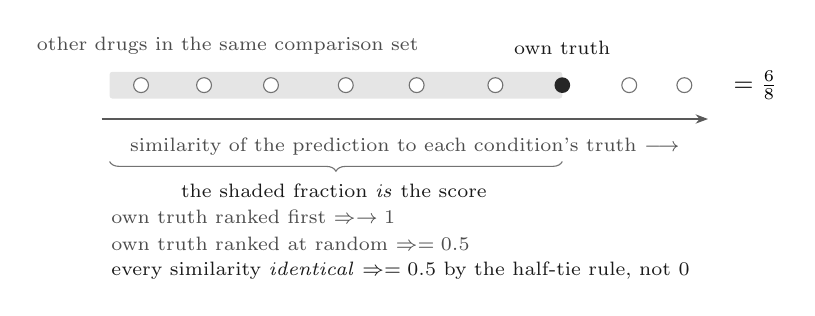
\begin{tikzpicture}[
  x=1cm, y=1cm, font=\small,
  lbl/.style={font=\scriptsize, text=black!70},
  strong/.style={font=\scriptsize, text=black!90},
  own/.style={circle, fill=black!85, inner sep=2pt},
  other/.style={circle, draw=black!55, fill=white, inner sep=1.9pt},
  ar/.style={-{Stealth[length=4.5pt]}, black!65},
]

\node[lbl, anchor=south] at (2.05,0.44) {other drugs in the same comparison set};
\node[strong, anchor=south] at (6.30,0.44) {own truth};

\fill[black!10, rounded corners=1pt] (0.55,0.00) rectangle (6.30,0.34);
\foreach \x in {0.95, 1.75, 2.60, 3.55, 4.45, 5.45} {\node[other] at (\x,0.17) {};}
\node[own] at (6.30,0.17) {};
\node[other] at (7.15,0.17) {};
\node[other] at (7.85,0.17) {};
\node[anchor=west, font=\small] at (8.35,0.17) {$\NIR = \tfrac{6}{8}$};

\draw[ar] (0.45,-0.26) -- (8.15,-0.26);
\node[lbl, anchor=north] at (4.30,-0.38)
  {similarity of the prediction to each condition's truth $\longrightarrow$};

\draw[decorate, decoration={brace, mirror, amplitude=3.5pt}, black!55]
  (0.55,-0.80) -- (6.30,-0.80);
\node[strong, anchor=north] at (3.40,-0.96) {the shaded fraction \emph{is} the score};

\node[lbl, anchor=west] at (0.45,-1.50) {own truth ranked first $\Rightarrow \NIR \to 1$};
\node[lbl, anchor=west] at (0.45,-1.84) {own truth ranked at random $\Rightarrow \NIR = 0.5$};
\node[strong, anchor=west] at (0.45,-2.18)
  {every similarity \emph{identical} $\Rightarrow \NIR = 0.5$ by the half-tie rule, not $0$};

\end{tikzpicture}
\caption[NIR is a discrimination score]{\textbf{$\NIR$ asks whether a prediction resembles its own
condition's truth more than it resembles the truths of the other drugs in the same comparison set.}
The generic response --- the stress and cell-cycle program every compound triggers --- is present in
every truth in equal measure, so it cancels in the comparison and only the drug-specific difference
decides. Two consequences follow, and both matter downstream. Chance at $0.50$ is a statement about
the \emph{comparison set}, not about the model: conditions are grouped by (cell line, plate) in the
expression frame and by cell line in the residual frame, and the two are not interchangeable. And a
predictor whose similarities are all identical --- the zero vector, which is what ``predict the
average drug response'' becomes in residual space --- must score $0.50$ rather than $0$, which is why
ties are counted at one half rather than dropped.}
\label{fig:nir}
\end{figure}


Finally, the metrics themselves need grading, and for that we port the framework of Miller
et al.~\cite{miller}, asking how well each \emph{metric} separates a positive from a negative
control:
\begin{equation}
  \DRF(m) \;=\; \frac{m(\textrm{pos}) - m(\textrm{neg})}{m(\textrm{perfect}) - m(\textrm{neg})},
\end{equation}
with $\textrm{pos}$ an interpolated-duplicate noise ceiling --- their positive control, which
interpolates a technical duplicate toward the mean baseline with per-gene weights given by
differential-expression significance --- and $\textrm{neg}$ a drug-agnostic leave-one-out mean. A
negative \DRF{} means the metric scores the uninformative baseline \emph{above} the noise ceiling:
it is inverted, and rewards the generic gene ordering rather than the drug. Three hardening choices
matter for how the result can be read. Tied expression values receive \emph{average} ranks, because
breaking ties by array index makes a tied gene's rank depend on its position in the panel. The
\DRF{} ratio is recomputed \emph{whole} inside every bootstrap resample, because its denominator is
estimated from the same data as its numerator and holding it fixed understates the interval. And
the family of five metrics is controlled simultaneously with Holm's procedure, because the claim
``only $\NIR$ is calibrated'' is a claim about all five at once.

Adopting this framework is deliberate. Miller et al.\ use it to argue that reports of deep models
failing to beat uninformative baselines reflect miscalibrated evaluation rather than model failure
(Section~\ref{sec:lit-dispute}). Evaluating our model on the metric \emph{their} analysis endorses
means the result reported in Section~\ref{sec:res-blind} cannot be dismissed on the grounds their
own paper raises.

\subsection{Controls}
\label{sec:methods-controls}

The negative results in this thesis are only as strong as the controls that make them
interpretable. Each of the following exists because a specific objection would otherwise be fatal,
and each is stated with the failure it closes.

Drug and plate are partially confounded by Tahoe's design: each drug is assayed on its own
plate(s), with roughly 4--12 drugs per plate and plate-matched controls. Discrimination grouped by
cell line alone therefore lets the \emph{batch} signature stand in for drug identity. Measured
directly, by scoring the same tier-2 conditions with and without the plate held constant:

\begin{table}[h]
\centering
\begin{tabular}{lrr}
\toprule
Predictor (drug-agnostic) & cross-plate & within plate \\
\midrule
mean baseline & 0.399 & \textbf{0.161} \\
control-copy & 0.551 & 0.510 \\
\midrule
noise ceiling & 0.625 & 0.575 \\
fraction of drugs at chance & 43\% & 49\% \\
\bottomrule
\end{tabular}
\caption{Expression-frame $\NIR$. A drug-agnostic mean baseline more than doubles its score when the
plate is free to vary, which is what plate leakage looks like. The ceiling falls once the plate is
held constant because the batch signature was inflating it too.}
\label{tab:plateleak}
\end{table}

The mean baseline is the clearest demonstration: it contains no drug information whatsoever, and it
scores $0.399$ when the comparison set may span plates against $0.161$ when it may not. Every
discrimination instrument therefore gained a \texttt{--same\_plate\_only} mode and all discrimination
results in this thesis were re-run within plate. Conclusions are unchanged; some magnitudes shrink.

A separate and stronger observation, which belongs to the drug-blindness argument rather than to this
one, is that \emph{within} plate and on the identifiable stratum a control-copy baseline reaches
$0.766$ against the model's $0.768$ (Section~\ref{sec:res-blind}). That is not a statement about
plate leakage --- it is a statement about the model.

\paragraph{The scramble ablation, and what its comparator must satisfy.} The central manipulation
leaves the prompt byte-identical except that the drug name and mechanism are replaced by another
drug's, while the control cell and the scoring truth are unchanged. Because both arms share the
same control cell, control- and batch-derived leakage cancels in the \emph{difference}
$\gap = \NIR_{\textrm{model}} - \NIR_{\textrm{scramble}}$. This is the only manipulation that
isolates drug use, and every drug-use claim in this thesis is anchored to it rather than to a
comparison against a drug-agnostic predictor.

Two constraints on the swap partner are required for a gap measured this way to mean what it says,
and both exist because the unconstrained pool fails in a specific way. The partner must be a
\emph{different drug}: allowing the same drug at another dose or plate substitutes the drug for
itself, an unchanged output is then correct rather than blind, and the contamination concentrates
in the most similar stratum because a drug's own other doses are usually its nearest neighbours.
And the partner must be on the \emph{same plate}: residuals retain plate structure, so a
cross-plate partner differs from the target in batch as well as in drug, and the gap absorbs both.

A scramble that swaps in a drug with a \emph{similar} true response is also a weak test, and this is
a real risk here because same-mechanism drugs are barely more similar than random pairs (within-MoA
distance $2.322$ versus between-MoA $2.377$, ratio $0.977$), so ``different mechanism'' does not
imply ``different response''. Two remedies are used: a \emph{swap-distance sweep} that turns the
single test into a curve of $\gap$ against the response distance $\lVert y_A - y_B \rVert$ between
the real and swapped-in drug; and a \emph{stratified scramble} with three defined partners per
condition chosen by residual cosine within the cell line --- \texttt{near} (most similar),
\texttt{orth} ($\cos\approx0$) and \texttt{opposite} (most anti-correlated). The strata make an
assumption visible that a single comparator hides: the gap has two parts, how much naming the truth
helps and how much naming a lie hurts, and only the first is wanted. A usable null is therefore a
stratum whose own score sits at chance --- which, Section~\ref{sec:res-generalisation} shows, is
true of exactly one of the three, and not the one an evaluation would naturally default to.

% fig-scramble.tex -- the scramble ablation and why its difference is leak-immune.
% No data dependency.
% Layout note: the prompt boxes are ~2.2cm tall once the shaded spans are set, which is far more
% than a four-line block looks like it should need. Every band below them is placed against that
% measured height, not against an estimate.
\begin{figure}[htbp]
\centering
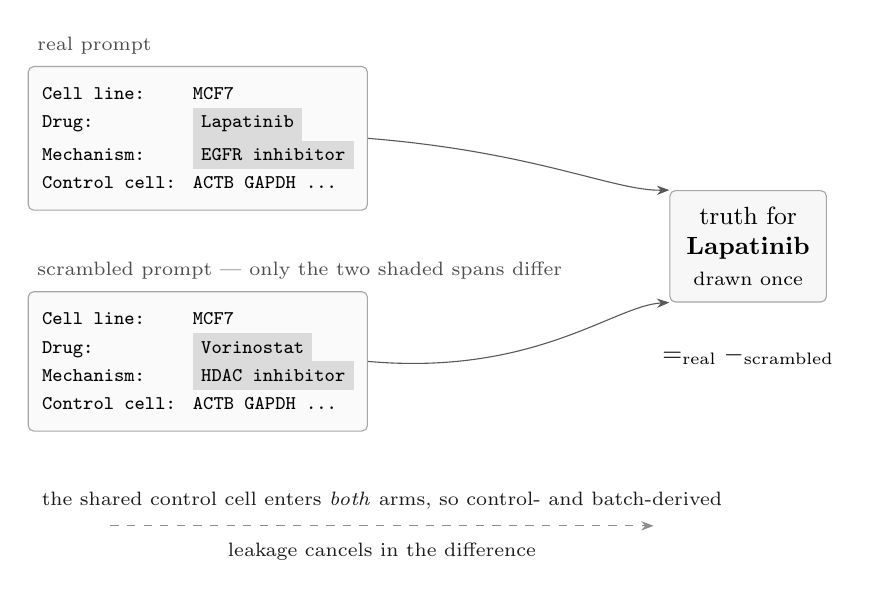
\begin{tikzpicture}[
  x=1cm, y=1cm, font=\small,
  lbl/.style={font=\scriptsize, text=black!70},
  strong/.style={font=\scriptsize, text=black!90},
  promptbox/.style={draw=black!35, rounded corners=2pt, inner sep=5pt, fill=black!2},
  ar/.style={-{Stealth[length=4.5pt]}, black!65},
]
\newcommand{\spanhl}[1]{\colorbox{black!14}{#1}}

\node[lbl, anchor=west] at (0.15,0.00) {real prompt};
\node[promptbox, anchor=north west] (p1) at (0.15,-0.26) {%
  \renewcommand{\arraystretch}{0.9}%
  \begin{tabular}{@{}l@{~~}l@{}}
  \ttfamily\scriptsize Cell line:    & \ttfamily\scriptsize MCF7 \\
  \ttfamily\scriptsize Drug:         & \ttfamily\scriptsize \spanhl{Lapatinib} \\
  \ttfamily\scriptsize Mechanism:    & \ttfamily\scriptsize \spanhl{EGFR inhibitor} \\
  \ttfamily\scriptsize Control cell: & \ttfamily\scriptsize ACTB GAPDH \ldots \\
  \end{tabular}};

\node[lbl, anchor=west] at (0.15,-2.86) {scrambled prompt --- only the two shaded spans differ};
\node[promptbox, anchor=north west] (p2) at (0.15,-3.12) {%
  \renewcommand{\arraystretch}{0.9}%
  \begin{tabular}{@{}l@{~~}l@{}}
  \ttfamily\scriptsize Cell line:    & \ttfamily\scriptsize MCF7 \\
  \ttfamily\scriptsize Drug:         & \ttfamily\scriptsize \spanhl{Vorinostat} \\
  \ttfamily\scriptsize Mechanism:    & \ttfamily\scriptsize \spanhl{HDAC inhibitor} \\
  \ttfamily\scriptsize Control cell: & \ttfamily\scriptsize ACTB GAPDH \ldots \\
  \end{tabular}};

\node[draw=black!35, rounded corners=2pt, inner sep=6pt, align=center, fill=black!3]
  (truth) at (9.30,-2.55) {truth for\\\textbf{Lapatinib}\\{\scriptsize drawn once}};

\draw[ar] (p1.east) .. controls (6.6,-1.35) and (7.6,-1.85) .. (truth.north west);
\draw[ar] (p2.east) .. controls (6.6,-4.20) and (7.6,-3.30) .. (truth.south west);

\node[anchor=north, font=\small] at (9.30,-3.70)
  {$\gap = \NIR_{\text{real}} - \NIR_{\text{scrambled}}$};

\draw[ar, dashed, black!45] (1.20,-6.10) -- (8.10,-6.10);
\node[strong, anchor=south, align=center] at (4.65,-6.02)
  {the shared control cell enters \emph{both} arms, so control- and batch-derived};
\node[strong, anchor=north, align=center] at (4.65,-6.20)
  {leakage cancels in the difference};

\end{tikzpicture}
\caption[The scramble ablation]{\textbf{The scramble replaces the drug name and its mechanism and
nothing else.} Both arms are conditioned on the same control cell and scored against the same truth,
so any leakage through the control cell or the plate enters both arms in equal measure and cancels in
the difference $\gap$. This is why $\gap$, rather than a comparison against a drug-agnostic
predictor, is the quantity every drug-use claim in this thesis is anchored to: the drug-agnostic
comparison is not leak-immune, and a drug-agnostic mean baseline scores $\NIR = 0.399$ when the
comparison set may span plates against $0.161$ when it may not, precisely because it inherits that
leakage. A refinement matters here and is
developed in Section~\ref{sec:methods-controls}: if the swapped-in drug happens to have a
\emph{similar} true response then an unchanged output is correct rather than blind, so the swap
partner is chosen from three defined similarity strata and the evidence is the \emph{gradient} across
them rather than any single value.}
\label{fig:scramble}
\end{figure}


The scramble replaces the drug name \emph{and} its mechanism together, so a non-null gap
establishes sensitivity to the combined drug-and-mechanism prompt without attributing it to either
span. A \emph{field decomposition} costs one extra pair of generation arms and swaps exactly one
span of the instruction line to the opposite-signature partner, leaving every other byte identical:
the drug name with the mechanism kept, the mechanism with the name kept, and both together. One
guard is essential rather than tidy. If the swap partner happens to share the original's mechanism,
then swapping only the mechanism produces a prompt \emph{identical} to the model's own, and the arm
scores a gap of exactly zero \emph{by construction}. Read naively that is indistinguishable from
``the model ignores the mechanism'', which is the very claim under test. Such conditions are
dropped rather than scored, which is why the mechanism arm carries fewer conditions than the others.

\paragraph{Two further drug-isolating instruments.} The drug-blindness claim rests on four
instruments rather than one, because they fail in different ways and agreement across them is worth
more than any single number. Two are defined above ($\NIR$ and the scramble); the other two are
forced-choice grading and output invariance.

In \emph{forced-choice grading}, a prediction is scored against its own condition's truth and
against another drug's truth from the same comparison set, and the instrument records how often the
own truth wins. Chance is $0.50$ by construction. The ceiling is the same forced choice with a real
held-out replicate substituted for the prediction, which bounds what any predictor could achieve at
this noise level; it lands between $0.67$ and $0.83$ depending on cells per condition.

\emph{Output invariance} asks whether the drug token changes the generated text at all, without
reference to any truth. For a fixed control cell, the model generates twice from the \emph{same}
prompt and once from each of several prompts differing only in the drug, and the instrument compares
\begin{equation}
  \textrm{gap} \;=\; \underbrace{\overline{\textrm{sim}}(\textrm{same prompt, resampled})}_{\textrm{sampling noise alone}}
  \;-\; \underbrace{\overline{\textrm{sim}}(\textrm{prompts differing in the drug})}_{\textrm{noise plus any drug effect}},
\end{equation}
with similarity measured as top-$100$ Kendall $\tau$ and as Jaccard overlap. A positive gap means two
generations for the same drug resemble each other more than generations for different drugs do,
i.e.\ the drug token moves the output. A gap of zero means swapping the drug perturbs the output no
more than resampling at the same temperature does. Reported over $8$ contexts $\times$ $12$ drugs at
temperature $0.8$. This instrument is the weakest of the four --- it can only detect whether the
output moves, not whether it moves \emph{correctly} --- but it is also the one least able to be
confounded, since it needs no ground truth at all.

\paragraph{Channel gate.} For an unseen drug, prediction is only possible through a property the drug
\emph{shares} with drugs seen in training, so the reachable channels can be enumerated and each one
measured in the same frame. For a channel $X$, a drug's residual is predicted as the mean residual of
the \emph{other} drugs in the same cell line that share property $X$ with it --- the construction of
the mechanism baseline, generalised. Because it uses only drugs that were in training, it is a fair
contest in every split, unlike a same-drug lookup, which on an unseen drug is an oracle.

The gate's estimand requires the channel arm and its null to differ in exactly one respect, and two
disciplines enforce it. Every channel is paired with a \textbf{plate-matched random null}: the same
\emph{number} of partner drugs, drawn at random from the same cell line, \emph{and} the same split
of partners across the target's own plate and other plates, because mechanism- and target-related
drugs are co-plated more often than chance --- a null matched on count alone would differ from the
channel arm in plate membership as well as in the channel, which is two differences where the
estimand allows one. A \textbf{co-plating diagnostic is printed before any verdict}, so the size of
the correction is a number rather than an argument, and where a plate-matched null spans too few
cell lines the channel is reported \textsc{untestable} rather than closed --- ``we could not build
the control'' must never be written as ``closed''. Coverage is likewise reported before any
verdict, because a channel annotated on few drugs cannot be closed by a null result: it was never
tested.

The bound this establishes is on \emph{similarity transfer} through each channel, not on any model.
A model could in principle combine channels or learn a non-smooth structure-to-response map that a
nearest-neighbour average cannot express. A leave-one-drug-out regression over all channels jointly
addresses the first. The second is bounded by sample size rather than by argument: at a few hundred
drugs, learning a non-smooth map is not feasible, so at this $n$ the lookup is effectively the bound.

\paragraph{Is the interaction learnable?} The transfer coefficient says how \emph{large} the
drug$\times$cell-line interaction is; it says nothing about whether anything could learn it. If a cell
line modulated drug responses in a consistent direction, that direction would be estimable from the
line's own cells and a conditional model would have a concrete target. Writing
$\kappa(d,c) = \resid(d,c) - \hat{\beta}(d)$, the test compares $\cos(\kappa(d,c), \kappa(d',c))$ for
different drugs in the \emph{same} cell line against the same quantity across \emph{different} cell
lines.

$\hat{\beta}$ must be estimated \textbf{leave-one-cell-line-out}. Estimated over all lines it would
contain $\resid(d,c)$ itself, and subtracting a mean containing its own term induces a $-1/(m-1)$
correlation that biases the signal arm downward \emph{by construction} --- which would make a
structured interaction look idiosyncratic, the exact error the test exists to avoid. Both arms are
disattenuated by $\kappa$'s own split-half reliability, since $\kappa$ is a difference of two noisy
quantities and is therefore noisier than the residual it comes from.

\paragraph{Uncertainty.} Conditions are not independent, and they are not independent in two
crossed ways at once. Two conditions from the same treated well share a physical assignment and a
batch --- one well holds about $49$ cell lines dosed together --- and two conditions from the same
cell line share the biology. Treating conditions as independent gives intervals that are too
narrow; here, about $1.3$ to $1.5$ times too narrow. Neither grouping alone captures the
dependence, and the tempting shortcut is actively misleading: clustering on the assignment unit
alone uses the \emph{larger} cluster count ($289$ wells against $\approx 50$ lines) and would
\emph{tighten} every interval while sounding more rigorous. All intervals in this thesis are
therefore two-way cluster-robust (Cameron--Gelbach--Miller),
\begin{equation}
  V \;=\; V_{\textrm{line}} \;+\; V_{\textrm{well}} \;-\; V_{\textrm{intersection}},
\end{equation}
where the intersection of the two groupings is the single condition, so $V_{\textrm{intersection}}$
is the ordinary independent-sampling variance; when the estimator goes non-positive in a finite
sample the wider one-way variance is used and the branch recorded. Because a cluster-robust
variance is asymptotic in the number of \emph{clusters}, not observations, the reference
distribution is Student's $t$ with degrees of freedom one less than the smaller cluster count ---
which matters where an arm spans only $25$ wells, and moves a borderline verdict. For statistics
computed over \emph{pairs} of conditions, such as the transfer coefficient, neither grouping
partitions the observations --- a pair belongs to two nodes at once --- so those intervals use the
Fafchamps--Gubert dyadic estimator, under which two pairs are dependent whenever they share either
member. This is the structure DrEval~\cite{dreval} identifies in this field more broadly, citing
Hurlbert's pseudoreplication~\cite{hurlbert}: hundreds of thousands of cells resolving to a few
hundred conditions over $50$ cell lines.

\paragraph{Generation validity.} Every generation-based evaluation reports the \ENDCELL{}/\DOWN{}
completion rate, the fraction of emitted symbols that are valid panel genes, and the duplicate rate,
before any score is quoted. This is not hygiene: a $600$-token generation cap silently truncated
$26\%$ of generations in an early run and \emph{halved} the measured effect. Every contrast is
additionally generated with a fixed per-(condition, arm) seed, so the two arms of a paired
comparison are not drawn from different points of one global stream.

\subsection{Mechanistic probing}
\label{sec:methods-probe}

To distinguish ``cannot represent the drug'' from ``represents but does not use it'', four
instruments are needed, and again each exists because its predecessor fails in an instructive way.

Per-layer \emph{linear probes} on the residual stream at the last prompt token, predicting drug
identity, establish whether the information is present at all. But the raw drug subspace is partly
a batch subspace --- probing dose and plate from \emph{inside} it recovers dose at $0.90$--$0.95$ ---
so a context subspace is built from the union of cell line, plate and dose, and the drug axis is
orthogonalised against it; every causal claim uses the purified subspace. Before any ``ablating the
drug does nothing'' result is trusted, a \emph{removal gate} requires the subspace to contain the
drug: the fraction of above-chance probe accuracy removed by projecting it out must exceed $0.8$,
without which the null is unfalsifiable. The \emph{causal test} then reads log-probabilities of the
teacher-forced true response clean, then re-reads them with a forward hook projecting the subspace
out at every position, taking the mean KL divergence over response tokens; measuring in logit space
rather than by generating removes the sampling-noise floor that made an earlier steering experiment
inconclusive.

\paragraph{The identity test, and two designs that failed before it.} Ablation shows a subspace
carries functional variance; it cannot show that the subspace's \emph{drug-specific content} is read.
Only a substitution can. Two attempts at one were retracted, and since the failures were instructive
they are stated rather than hidden.

The first overwrote drug A's code with drug B's inside a purified subspace and compared the resulting
KL against a random vector of identical norm drawn in the \emph{full} residual stream --- so almost
all of the control's energy lay in directions the intervention never touched. The second drew the
random vector inside the subspace, which appeared to fix it and did not: the hook ablates before
adding, so the delivered perturbation is (added $-$ removed), and because the injected class mean was
uncentred it shared its global-mean component with the thing removed. The substitution arm was then
a near-restore and the control arm a genuine displacement. Simulated with no model in the loop, the
control delivers $5.3\times$ the perturbation in $100\%$ of draws. Both retracted results pointed the
same way, and that way was geometry rather than biology.

The design used here removes the ablation from the identity test. It injects a \emph{displacement}
$P(\mu_B - \mu_A)$ --- in which the global mean cancels exactly --- and scores a \emph{contrast},
\begin{equation}
  \log P\!\left(r_B \mid \textrm{prompt}_A\right) \;-\; \log P\!\left(r_A \mid \textrm{prompt}_A\right),
\end{equation}
so that any shift common to both responses, including the entire normaliser, subtracts out. What
survives is the model's preference between drug B's own held-out response and drug A's. The headline
control is a second real drug displacement $P(\mu_C - \mu_A)$, rescaled to identical norm: same
anchor, same construction, wrong drug. An isotropic in-subspace direction is retained only as an
off-manifold damage diagnostic, never as the comparison, because a random direction disrupts the
model in ways an on-manifold class-mean displacement does not.

Subspaces and class means are fit on one split, $r_B$ drawn from a second disjoint split, and all
scoring done on a third. Uncertainty is a cluster bootstrap over (A,B) pairs; equivalence requires
the interval to lie inside a pre-registered margin \emph{and} contain zero; and a layer is excluded
where the cell-line positive control has no dynamic range, since a saturated instrument cannot
support either verdict.

\subsection{Target constructions}
\label{sec:methods-targets}

The three target families below are attempts to fix the target \emph{content} while leaving its
encoding alone; Section~\ref{sec:res-epsilon} shows why that family of fix could not work, and the
ladder construction is what makes that demonstration conclusive rather than anecdotal.

\emph{Consensus.} Cells grouped by (drug, cell line, dose) and averaged into one pseudobulk
sentence, with every original prompt retained so only the response changes.

\emph{Optimal transport.} For each (cell line, plate) group, a coupling $\pi$ between control
and treated cells minimising $\sum_{ij}\pi_{ij}\lVert x_i - y_j\rVert^2$ under uniform marginals,
solved by Sinkhorn iteration~\cite{cuturi} on $K = \exp(-C/\varepsilon)$. Couplings are computed in
the released Tahoe scVI latent~\cite{scvi} ($n_{\textrm{latent}} = 10$), joined per cell by barcode
rather than re-encoded --- a re-encode produced a degraded latent (cell-line probe $0.11$ versus
$0.975$ for the shipped latent). Targets are built \emph{decoder-free}, as convex combinations of
real treated cells in expression space, so they always lie on the data manifold.

The regularisation parameter defines a ladder whose endpoints are experiments we had already run:
$\varepsilon\rightarrow\infty$ gives a uniform coupling and hence the treated mean (consensus);
$\varepsilon\rightarrow 0$ gives near-hard assignment, approximately a single state-matched treated
cell. This is what makes the sweep conclusive rather than anecdotal.

\subsection{Residual targets}
\label{sec:methods-residual}

The residual target asks the model to predict only what makes \emph{this} drug different. For each
condition (drug, cell line, plate, dose) with at least $40$ treated and $20$ plate-matched control
cells:
\begin{equation}
  \resid(d,c) \;=\; \underbrace{\big(\bar{y}_{\textrm{treated}} - \bar{y}_{\textrm{control}}\big)}_{\shift(d,c)}
  \;-\; \underbrace{\frac{1}{|D_c|}\sum_{d' \in D_c} \shift(d',c)}_{\textrm{generic}(c)} .
\end{equation}
The control subtraction removes the cell's own state; the mean-over-drugs subtraction removes the
\emph{generic drug program} --- the stress and cell-cycle response common to all compounds, which
Section~\ref{sec:res-metrics} shows accounts for essentially all of the model's apparent skill. What
remains is what makes \emph{this} drug different. Four properties of how the generic is estimated
decide whether that remainder can be trusted, and each was forced by a measured failure.

First, \textbf{the split precedes the fit}. An earlier build estimated the generic and the
reliability filter over \emph{every} condition and assigned the holdout afterwards, so each held-out
target was defined partly by other held-out conditions. The pipeline is therefore staged ---
inventory (metadata only), split (metadata only, before any pseudobulk exists), fit (the generic is
handed the training keys explicitly), transform (held-out conditions are projected through the
fitted generic and never enter it) --- and a poison test stands behind the staging: corrupting every
held-out expression vector must leave the training targets byte-identical, and corrupting a training
condition must change them.

Second, \textbf{the scope is the plate, not the cell line}. The original argument for cell-line
scope was reproducibility --- $62\%$ of conditions reproduce across a half-split at cell-line scope
against $19\%$ at plate scope, on the reasoning that a plate holds too few drugs to estimate a mean
and subtracting a noisy one injects noise. That comparison does not hold up: both figures were
computed with a \emph{shared} control pseudobulk subtracted from both halves, which makes the halves
correlate through their common control error, and the inflation is not neutral between scopes ---
it favours cell-line scope precisely because the cell-line generic is itself less noisy. Measured
with disjoint control halves, the two are comparable: $20\%$ at plate scope against $16\%$ at
cell-line scope. Two further diagnostics settle it in plate's favour and are reported in
Section~\ref{sec:res-transfer}: at cell-line scope the dose-transfer ordering inverts and the
shared-minus-split control bias reads $+0.254$, against $-0.000$ at plate scope. A plate group with
fewer than three other training drugs yields no generic, and the condition is dropped and counted
rather than silently falling back to the contaminated frame.

Third, \textbf{the mean is over drugs, not conditions}, and \textbf{leaves the condition's own drug
out}. A drug measured at five doses would otherwise contribute five times the weight of a
single-dose drug. And once the generic is train-only, an asymmetry appears that had not existed
before: a training condition's generic would contain its own drug while a held-out condition's would
not, so the two splits would be scored against differently defined targets and the generalisation
gap would partly measure that difference. The generic for every condition is therefore ``the mean
over training drugs other than this one, within scope'' --- identical in definition on both sides.

Fourth, \textbf{the reliability line is resolved from the data, not inherited}. A condition is kept
for training only if its residual reproduces across a half-split, $\cos(\resid_A, \resid_B)$ above
a threshold --- with each half measured against its \emph{own} control half, so the two share
nothing. The threshold itself was the single largest determinant of the training set, and it had
been inherited ($0.2$) from an era when reliability was measured with shared controls --- a
different quantity on a different scale, under which the mean is $\approx 0.6$ rather than
$+0.127$. Rather than pick a new number, the builder reports the whole retention curve against a
null that pairs half A of one condition with half B of a \emph{different} condition --- same
encoding, same dimensionality, same noise, no shared biology --- and the threshold is set at the
null's $95$th percentile: a condition is kept when its two halves agree more than two unrelated
conditions' halves do. At the measured null ($95$th percentile $+0.109$) this retains $2{,}523$ of
$4{,}999$ training conditions ($50.5\%$). The held-out sets are \emph{not} filtered by this
criterion: dropping held-out conditions for failing their own reproducibility bar would select the
evaluation set on its own outcome, so noise in retained training conditions costs learning
efficiency, not validity.

What this fraction means is stated carefully, because it is easy to over-read. The half-split
agreement is a \emph{within-well sampling-precision} criterion: it asks whether two disjoint cell
subsets of the \emph{same} well give the same residual. It is not biological reproducibility ---
$286$ of $287$ distinct (drug, dose) treatments in this atlas occur in exactly one well, so no
independent-well replicate exists to measure that with --- and the $50.5\%$ is a statement about
how much drug-specific signal survives pseudobulk noise at this cell budget, not about how much
biology is real.

\paragraph{Encoding and scoring.} The target string is
\texttt{<up genes> \DOWN{} <down genes> \ENDCELL}, $100$ genes per block, ordered by signed residual
magnitude; sign is biology, so it is given a symbol rather than being folded into a magnitude
ranking. Predicted and true residuals are both mapped to a signed rank vector (top-$k$ up positive,
top-$k$ down negative, weight $1/\log_2(\textrm{rank}+1)$) so a generated sentence and a continuous
truth are compared like for like; similarity is cosine and the score is $\NIR$ over other drugs in
the same cell line.

% fig-frame.tex -- the residual frame and the encoding fork.
% No data dependency. Annotations from RESULTS/target_divergence.json, cellline scope:
%   full 34.59 / shift 111.42 / residual 118.25 ; ceilings 0.7420 / 0.7420 / 0.7432.
% Layout notes:
%   * two subtraction ROWS, not an L-shape (the L put the generic term on a band that collided
%     with its own caption).
%   * the caption for the generic sits BELOW both rows, not between them -- between them it ran
%     under the divider and into the right-hand column.
%   * row labels are centred on profiles spaced 1.65cm apart; at 1.45cm "generic(c)" and
%     "residual r(d,c)" touch.
\begin{figure}[htbp]
\centering
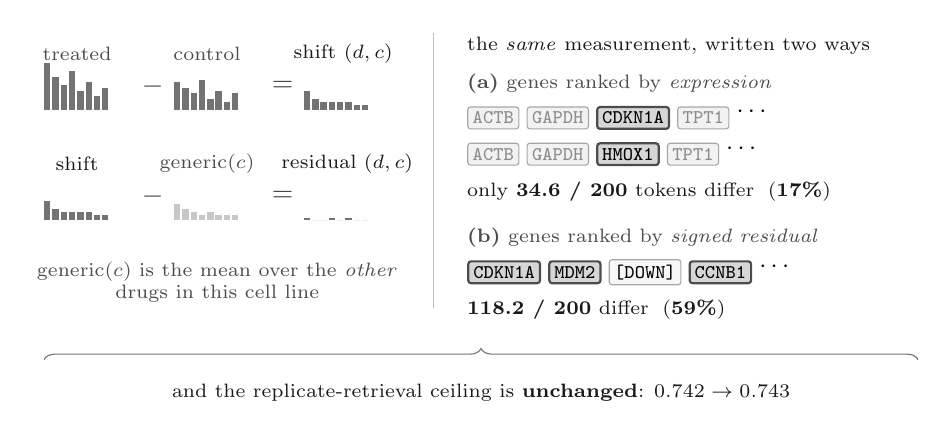
\begin{tikzpicture}[
  x=1cm, y=1cm, font=\small,
  bar/.style={fill=black!55, draw=none},
  faintbar/.style={fill=black!22, draw=none},
  gene/.style={draw=black!35, rounded corners=1pt, inner sep=1.8pt, font=\ttfamily\scriptsize},
  shared/.style={gene, fill=black!5, text=black!45},
  differs/.style={gene, fill=black!16, text=black, draw=black!70, thick},
  lbl/.style={font=\scriptsize, text=black!70},
  strong/.style={font=\scriptsize, text=black!90},
  op/.style={font=\normalsize, text=black!75},
]
\newcommand{\prof}[4]{%
  \foreach \h [count=\i from 0] in {#3} {
    \fill[#4] ($(#1,#2)+(\i*3.0pt,0)$) rectangle ++(2.3pt,\h pt);
  }%
}

% ================================================ LEFT: two subtractions
\node[lbl]    at (0.52,3.34) {treated};
\node[lbl]    at (2.17,3.34) {control};
\node[strong] at (3.90,3.34) {shift $\shift(d,c)$};
\prof{0.10}{2.62}{17,12,9,14,7,10,5,8}{bar}
\node[op] at (1.48,2.92) {$-$};
\prof{1.75}{2.62}{10,8,6,11,4,7,3,6}{bar}
\node[op] at (3.13,2.92) {$=$};
\prof{3.40}{2.62}{7,4,3,3,3,3,2,2}{bar}

\node[strong] at (0.52,1.94) {shift};
\node[lbl]    at (2.17,1.94) {generic$(c)$};
\node[strong] at (3.95,1.94) {residual $\resid(d,c)$};
\prof{0.10}{1.22}{7,4,3,3,3,3,2,2}{bar}
\node[op] at (1.48,1.52) {$-$};
\prof{1.75}{1.22}{6,4,3,2,3,2,2,2}{faintbar}
\node[op] at (3.13,1.52) {$=$};
\prof{3.40}{1.22}{1,0,0,1,0,1,0,0}{bar}

\node[lbl, anchor=north, align=center] at (2.30,0.82)
  {generic$(c)$ is the mean over the \emph{other}\\drugs in this cell line};

\draw[black!25] (5.05,0.10) -- (5.05,3.60);

% ================================================ RIGHT: the encoding fork
\node[strong, anchor=west] at (5.35,3.44) {the \emph{same} measurement, written two ways};

\node[lbl, anchor=west] at (5.35,2.96) {\textbf{(a)} genes ranked by \emph{expression}};
\node[anchor=west] at (5.35,2.52) {%
  \tikz[baseline]{\node[shared]{ACTB};}\;\tikz[baseline]{\node[shared]{GAPDH};}\;%
  \tikz[baseline]{\node[differs]{CDKN1A};}\;\tikz[baseline]{\node[shared]{TPT1};}\;$\cdots$};
\node[anchor=west] at (5.35,2.06) {%
  \tikz[baseline]{\node[shared]{ACTB};}\;\tikz[baseline]{\node[shared]{GAPDH};}\;%
  \tikz[baseline]{\node[differs]{HMOX1};}\;\tikz[baseline]{\node[shared]{TPT1};}\;$\cdots$};
\node[strong, anchor=west] at (5.35,1.58)
  {only \textbf{34.6 / 200} tokens differ \;(\textbf{17\%})};

\node[lbl, anchor=west] at (5.35,1.00) {\textbf{(b)} genes ranked by \emph{signed residual}};
\node[anchor=west] at (5.35,0.56) {%
  \tikz[baseline]{\node[differs]{CDKN1A};}\;\tikz[baseline]{\node[differs]{MDM2};}\;%
  \tikz[baseline]{\node[gene, fill=black!3]{[DOWN]};}\;\tikz[baseline]{\node[differs]{CCNB1};}\;%
  $\cdots$};
\node[strong, anchor=west] at (5.35,0.08)
  {\textbf{118.2 / 200} differ \;(\textbf{59\%})};

% ================================================ the invariant
\draw[decorate, decoration={brace, amplitude=4pt}, black!55] (0.10,-0.55) -- (11.20,-0.55);
\node[strong, anchor=north] at (5.65,-0.73)
  {and the replicate-retrieval ceiling is \textbf{unchanged}: $0.742 \rightarrow 0.743$};

\end{tikzpicture}
\caption[The residual frame and the encoding fork]{\textbf{The information was always present; the
tokenisation discarded it.} Left: the drug-specific residual is built by two subtractions. The
control removes the cell's own state, leaving the \emph{shift}; the mean over the other drugs in the
same cell line removes the \emph{generic} program that every compound triggers, leaving what makes
this drug different. Right: that same measurement, written two ways. Ranking genes by expression (a)
puts housekeeping genes first, so only $34.6$ of the top $200$ tokens differ between two drugs in the
same context and cross-entropy has almost nothing to learn drug identity from; ranking by signed
residual (b) raises that to $118.2$. The bracket is the point of the figure --- the
replicate-retrieval ceiling is essentially identical under both encodings, so no information has been
added. What changed is how much of it the token sequence exposes to the loss.}
\label{fig:frame}
\end{figure}


\subsection{Generalisation design}
\label{sec:methods-holdout}

This is the choice on which every generalisation claim in the thesis stands or falls, and it is
forced by the physical design of the atlas rather than by statistics. Tahoe applies one drug at one
dose to one well containing $\approx 49$ cell lines simultaneously --- measured: $289$ treatment
samples, a mean of $48.6$ cell lines per well (median $49$, range $43$--$50$), and $286$ of $287$
distinct (drug, dose) treatments occurring in exactly one well. Three consequences follow, and they
apply to every analysis of this atlas, not only this one.

A drug cannot be present in cell line A and absent from cell line B at the same dose, because the
two lines are physically the same well. So a $(\textrm{drug}, \textrm{cell line})$ holdout --- the
field's standard Leave-Pairs-Out split, and the split an earlier version of this work used ---
leaves the held-out condition's treated well sitting in the training set through its other
$\approx 48$ cell lines. Measured against the holdout this thesis previously used, $124$ of the
$268$ treated wells in this cache placed a held-out condition and a training condition in the same
physical sample. What that estimand measures is \emph{within-atlas matrix completion}, not
independent generalisation, and no processing of the targets changes it, because it is a property
of what was randomised.

Holding out \emph{whole wells} is the only assignment-respecting choice the design offers, and it
answers a different and narrower question: generalisation to an \emph{unseen treatment well of a
seen drug} --- a new physical preparation, not a new cellular context. Fixed-dose cross-context
transfer, present in one line and absent in another, is structurally unidentifiable in this atlas;
this is a property of Tahoe's design, not of our pipeline, and no rebuild fixes it. The split used
throughout the residual arm is therefore keyed at the well:
\begin{description}
  \item[\texttt{train}] every condition of the remaining wells ($4{,}999$ conditions before the
        reliability line, $2{,}523$ after it).
  \item[\texttt{unseen\_combo} --- unseen wells of seen drugs] $36$ treated wells held out whole
        ($904$ conditions, $900$ after inventory filters). The holdout never takes a drug's last
        training well --- without that guard a two-well drug could silently become an unseen
        \emph{drug} while sitting in the unseen-combination arm, making the two arms measure the
        same thing. Zero wells contribute conditions to both sides of this split.
  \item[\texttt{unseen\_drug} --- Leave-Drugs-Out] every condition of $10$ held-out drugs ($714$
        conditions, $711$ after inventory filters). The model never sees the token. This is the
        \emph{control}: naming a drug the model knows nothing about versus naming something else can
        make no difference, so the measured effect there must be zero --- a non-zero value is an
        instrument fault, not a biological finding.
\end{description}

We do not build a Leave-Cell-Lines-Out (LCO) split here; Section~\ref{sec:limitations} argues it is
the natural next axis and explains why its interest is contingent on the transfer coefficient.

\paragraph{A warning we inherit with the vocabulary.} DrEval reports, citing~\cite{partin}, that
apparently good performance on pair-holdout splits can be reached simply by predicting each drug's
average response across the training cell lines. Our held-out-well estimand sits exactly in the
regime where that warning bites: the drug is seen, and its average is computable. This is the
reason the baseline ladder below is not optional: the drug-average predictor is not a formality to
be dismissed, it is the hypothesis under test.

\paragraph{Stratified sampling.} Evaluation samples conditions under an explicit per-split quota. A
uniform draw reproduces the pool's proportions, which starves precisely the split the experiment
exists to test: in a first run, $250$ constructed held-out combinations yielded only $33$ scored
conditions, purely as an artifact of the sampler. The residual-frame evaluation therefore scores
$200$ train, $250$ \texttt{unseen\_combo} and $120$ \texttt{unseen\_drug} conditions --- the latter
two being quotas of the $900$ and $711$ available, so the held-out verdicts in
Section~\ref{sec:res-generalisation} are powered on a subset of the conditions the split affords,
and their detection limits should be read with that in mind.

\subsection{Baselines}
\label{sec:methods-baselines}

Each baseline is a predictor of the drug-specific residual, scored through an identical pipeline ---
same truths, same signed-rank encoding, same comparison set.

\begin{table}[h]
\centering
\begin{tabular}{lll}
\toprule
Baseline & Information used & Role \\
\midrule
\texttt{drug\_lookup}   & this drug's mean residual, all other cell lines & the bar to beat \\
\texttt{drug\_lookup\_1} & this drug in \emph{one} other cell line & removes the averaging advantage \\
\texttt{moa\_lookup}    & other drugs sharing this drug's MoA, same cell line & mechanism-leak diagnostic \\
\texttt{control\_copy}  & none (predict the control cell) & must be $\approx 0.50$ \\
\texttt{generic}        & none (predict the average response) & must be $\approx 0.50$ \\
\texttt{random}         & none & floor \\
\bottomrule
\end{tabular}
\caption{The baseline ladder. \texttt{drug\_lookup} is the pre-registered win condition: a lookup
can reproduce a memorised average, so only a model that tailors the response to the control cell's
state can beat it.}
\label{tab:baselines}
\end{table}

Two disciplines make the ladder fair. The lookups are fitted from \textbf{training conditions
only}: fitted from the full cache, a lookup scoring a held-out condition reads residuals the model
was never shown --- an oracle, not a baseline --- and the oracle variants are reported alongside,
explicitly labelled, as a bound on how much the comparison was ever inflated rather than hidden.
And \texttt{drug\_lookup\_1} selects a cell \emph{line} and averages that line's conditions rather
than selecting a single condition, because $62\%$ of drugs are multi-dose and a single condition
would confound ``different cell line'' with ``different dose''. \texttt{moa\_lookup} is not an
oracle in any split, as it uses only drugs that were in training.

\subsection{Variance decomposition}
\label{sec:methods-vardecomp}

To separate the per-drug main effect from the drug$\times$cell-line interaction we model
\begin{equation}
  \resid(d,c) \;=\; \beta(d) \;+\; \kappa(d,c) \;+\; \epsilon,
  \qquad
  \Tcoef \;=\; \frac{\operatorname{var}\beta}{\operatorname{var}\beta + \operatorname{var}\kappa},
\end{equation}
where $\beta$ is constant across cell lines and $\kappa$ is the interaction --- the only component a
conditional model can win on.

\paragraph{This is DrEval's naive predictor, in transcriptomic space.} DrEval's
\texttt{NaiveMeanEffectsPredictor}~\cite{dreval} predicts
$\hat{y}_{ij} = \mu + (\mu^c_i - \mu) + (\mu^d_j - \mu) = \mu^c_i + \mu^d_j - \mu$: an additive
model of cell-line and drug main effects, with no interaction term. Our
$\textrm{generic}(c) + \beta(d)$ is precisely that quantity, lifted from a scalar potency to a
$946$-dimensional profile. It follows that $\kappa$ \emph{is} the term their naive model omits, and
that $1 - \Tcoef$ measures exactly the headroom available above it. DrEval finds that deep models
barely beat this additive baseline on drug sensitivity; the transfer coefficient asks whether, in
the transcriptomic setting, there is anything above it to win in the first place.

$\Tcoef$ is estimated by disattenuated cross-line correlation,
\begin{equation}
  \hat{\Tcoef} \;=\; \frac{\cos\!\big(\resid(d,c_1),\, \resid(d,c_2)\big)}
                           {\sqrt{\rho(d,c_1)\,\rho(d,c_2)}},
  \qquad
  \rho \;=\; \frac{2\cos(\resid_A, \resid_B)}{1 + \cos(\resid_A, \resid_B)},
\end{equation}
with $\rho$ the Spearman--Brown reliability of the full-sample residual. Dividing out the
reliability is essential --- measurement noise alone depresses the raw cross-line cosine and would
otherwise be read as interaction --- and the reliability entering it is a \emph{within-well}
split-half precision, which is optimistic relative to true biological reproducibility. That
optimism sits in the denominator, so the interaction share $1 - \Tcoef$ is, if anything,
understated.

Five controls accompany the estimate, each capable of changing the conclusion:
\begin{enumerate}
  \item \textbf{Control half-split.} Subtracting one shared control pseudobulk from both halves
        leaves control-estimation error common to $\resid_A$ and $\resid_B$, inflating the
        reliability and biasing $\Tcoef$ \emph{downward} --- manufacturing apparent interaction.
        Both builds are run and the bias reported ($+0.254$ at cell-line scope, $-0.000$ at plate
        scope).
  \item \textbf{Negative control, structure-matched.} A different drug in a \emph{different} cell
        line, breaking only the drug match while preserving the cross-line structure of the
        estimand; it must read $\approx 0$. A same-plate/different-drug control was tried first and
        is \emph{not} adequate: it differs from the estimand in two ways at once, and plate
        structure surviving a cell-line-scoped generic inflates it to $+0.478$ while leaving the
        estimand untouched --- which produced a false-alarm rejection before the matched control was
        built.
  \item \textbf{Simulated null.} At $\kappa = 0$ the estimator does not return $1.0$. A simulation
        calibrated to the measured noise level fixes the reference. In validation the raw cross-line
        cosine at $\kappa = 0$ is $0.734$, which read naively reports $27\%$ interaction where the
        truth is zero.
  \item \textbf{Dose strata.} Same drug, same cell line, different dose is not cross-line transfer;
        it is reported separately as a reference scale, with dose resolved to a \emph{molar}
        quantity --- an earlier cache carried the well identifier in the dose field, so what was
        labelled dose transfer compared physical samples rather than concentrations.
  \item \textbf{Leave-one-out generic.} The generic includes drug $d$, leaving a $-1/m$ self-term,
        unless the condition's own drug is excluded --- which, per
        Section~\ref{sec:methods-residual}, it now is.
\end{enumerate}
Validation against planted ground truth recovers $\Tcoef = 1.00$, $0.70$ and $0.40$ to within
$0.005$, and the different-drug negative control returns $-0.001$.

Finally, an exact energy decomposition of the shift into residual, generic and their cross term ---
the three shares sum to one by construction --- reports what fraction of the total perturbation
response the drug-specific frame covers: the number that scopes every claim in this thesis, and one
that has not previously been computed for this task.

\section{Results and Analysis}
\label{sec:results}

This chapter makes one argument in five moves, and the order is load-bearing. The field's standard
metric is shown to be gameable before any model is scored, because every later claim depends on the
ruler. Under a ruler that cannot be gamed, the model is drug-blind, and the blindness is located in
what the model is asked to predict rather than in what it can represent. Re-encoding the prediction
target then produces genuine prompt sensitivity --- and the chapter's central result is that this
sensitivity does not become reliable held-out prediction: a training-only lookup table beats the
model decisively, and the gap between the two is where the thesis ends.

\subsection{The metric is the first result}
\label{sec:res-metrics}

Before asking what the model knows, we have to know what the scoreboard rewards. The answer, for
the field's default metric, is: nothing about the drug. A predictor that places every gene at the
middle rank --- carrying no information about drug, cell or biology --- scores $\DEdr(K{=}50) =
0.9999$ [$0.99991$, $0.99992$], above the two-real-cell noise ceiling ($0.76$) and above the model
($0.73$). The ordering is inverted: less information yields a higher score, which is the signature
of an artefact rather than of skill. The same predictor's partial-$\DEdr$ and $\paneltau$ are
\emph{undefined} rather than merely poor --- its shift from control is identically zero, so there
is nothing left to correlate once the control is regressed out. The cause is exactly the mechanism
Section~\ref{sec:methods-metrics} flagged: $\DEdr$ selects the scored genes using the truth, and a
prediction that reverts toward the centre correlates with the true change by construction.

\begin{table}[h]
\centering
\begin{tabular}{lrrr}
\toprule
Predictor & Information & $\DEdr$ (K50) & partial-$\DEdr$ \\
\midrule
\texttt{revert\_center} (all genes $\rightarrow P/2$) & none & \textbf{0.9999} & undefined \\
\texttt{revert\_mean} (predict mean control) & none, no fit & 0.961 & 0.25 \\
ridge linear (control $\rightarrow$ shift) & control & 0.947 & 0.28 \\
noise ceiling (two real cells) & --- & 0.76 & --- \\
model (1B LLM) & control + drug & 0.73 & not measured \\
\bottomrule
\end{tabular}
\caption{$\DEdr$ is saturated by a control artefact. Regressing the control out of the two fitted
baselines leaves $\approx 0.26$ of real but \emph{drug-agnostic} skill, and a baseline that performs
no fitting at all reaches the same figure. The model's own partial-$\DEdr$ was never computed --- it
requires a GPU pass that was not run --- so the cell is marked rather than filled with the expected
value; the model's $\paneltau$, which \emph{is} measured, carries the same conclusion below.}
\label{tab:de-artifact}
\end{table}

Removing the control (partial-$\DEdr$) collapses the raw $0.95$ to $\approx 0.26$ for the two
baselines that were scored --- and that residue is matched by a baseline that performs no fitting at
all. The model's own partial-$\DEdr$ is not measured, so the comparison is anchored instead to
$\paneltau$, which is measured for every arm and tells the same story: \texttt{revert\_mean} $0.268$,
ridge $0.265$, model $0.257$ (tier 2, \texttt{worst} convention). The response decomposes into
control reversion (an artefact), a generic drug program ($\approx 0.26$, drug-agnostic, trivially
matched), and a drug-specific component that no predictor captures.

Grading the five metrics against each other settles which instrument the rest of the thesis may
use. Under the hardened \DRF{} protocol of Section~\ref{sec:methods-metrics} --- tie-aware ranks,
the ratio resampled whole, the family controlled by Holm's procedure --- $\NIR$ is the only
calibrated metric: $\DRF = \ci{+0.635}{+0.618}{+0.652}$, Holm $p = 0.0025$. The four rivals remain
strongly negative and none approaches significance (Holm-adjusted $p = 1.0000$ for all four); in
the earlier unhardened calibration they read $-0.081$ (\texttt{weighted\_r2}), $-0.231$
($\paneltau$), $-0.415$ (\texttt{spearman\_expr}) and $-0.448$ ($\DEdr$), and a negative \DRF{}
means the metric scores a drug-agnostic baseline \emph{above} the noise ceiling. The inversion is a
property of the data, not a leak: a leave-one-out correction barely moves the numbers, since real
cell lines carry 20--204 drugs, and it survives holding the plate constant.

This replicates Miller et al.\ --- and then diverges from them. Their central methodological claim
is confirmed emphatically: metric choice dominates, the rank-based metric is the one that survives,
and the correlation-based metrics they identify as poorly calibrated are exactly the ones that fail
here. The agreement extends to the specific metrics --- they find $\NIR$ consistently calibrated
across 14 Perturb-seq datasets, and we find it is the only calibrated metric of the five we tested
on drug perturbation. Our \texttt{weighted\_r2} result is also consistent with their finding that
weighted metrics behave better than unweighted ones. The divergence comes at the next step. Miller
et al.\ conclude that under calibrated metrics deep models outperform uninformative baselines;
Section~\ref{sec:res-blind} evaluates on the calibrated metric and finds the model at chance. Two
differences in setting are candidates for the discrepancy --- genetic versus drug perturbation, and
a discriminative regression model versus an autoregressive generative one --- and
Section~\ref{sec:res-lookup} supplies a third and more structural possibility.

\begin{figure}[htbp]
\centering

\includegraphics[width=\textwidth]{fig-calibration}
\caption[The standard metric is exploitable]{\textbf{Under the standard metric, less information
yields a higher score.} (a) A predictor that places every gene at the middle rank --- carrying
nothing about drug, cell or biology --- scores $\DEdr = 0.9999$, above the two-real-cell noise
ceiling and above both the model and its own scramble. The inverted ordering is the signature of an
artefact rather than of skill, and its cause is control regression-to-the-mean. Tier 2, $n=400$
conditions. No intervals are drawn: the stored ones are normal approximations rather than the
cell-line-clustered bootstraps used everywhere else in this thesis, and mixing the two conventions
on one axis would misrepresent both. (b) Grading the \emph{metrics} rather than the models. The
displacement drawn is the Dynamic Range Fraction, on a scale where $0$ is the drug-agnostic baseline
and $1$ a perfect predictor, so a negative value means the metric ranks an uninformative baseline
\emph{above} the noise ceiling. Only $\NIR$ points forward; the hardened estimate is
\ci{+0.635}{+0.618}{+0.652}. $655$ drugs over $61$ cell-line$\times$plate
groups, within plate. \texttt{weighted\_r2} carries no directional claim --- its sign tracks cell
count, and it is approximately neutral.}
\label{fig:calibration}
\end{figure}

The metric can discriminate even if the model cannot: a spike-in forced choice between two real
drug populations separates them essentially perfectly at pseudobulk ($\paneltau = 1.000$, $\DEdr =
0.995$, top-$n$ $\tau = 0.987$, plate held constant). The instrument is not the bottleneck.

\subsection{The model is drug-blind}
\label{sec:res-blind}

Having established which instrument can be trusted, we can finally ask the question the thesis
exists to answer. The answer is uniform across four instruments that fail in different ways, which
is the only reason to report all four.

\begin{table}[h]
\centering
\begin{tabular}{lrl}
\toprule
Instrument & Value & Reading \\
\midrule
Forced-choice grading & $0.48$ ($\approx$ scramble; ceiling 0.67--0.83) & chance \\
Output invariance (gap) & \ci{0.000}{-0.019}{+0.016} & null \\
Scramble $\DEdr$, tier 1 & $0.740$ real vs $0.739$ scrambled & identical \\
Scramble $\DEdr$, tier 2 & $0.733$ real vs $0.729$ scrambled & identical \\
$\gap$ (identifiable subset) & \ci{+0.014}{-0.016}{+0.042} & null \\
\bottomrule
\end{tabular}
\caption{Four independent instruments agree. Near-ceiling $\DEdr$ is achieved \emph{identically}
with a wrong-mechanism drug, so the score is drug-independent.}
\label{tab:blind}
\end{table}

Before asking what the model knows, it is worth asking what there is to know. A ladder of
mean-shift baselines --- each predicting the average response of a progressively narrower group ---
answers that directly. On tier 2, predicting the global mean scores $\DEdr$ $0.056$; conditioning
on cell line roughly triples it to $0.142$; conditioning on mechanism does not move it ($0.052$);
and conditioning on mechanism \emph{and} cell line is no better than cell line alone ($0.120$
against $0.142$). Tiers 1 and 3 tell the same story. The informative conditioning variable in this
data is therefore the cellular context, not the compound class --- worth holding onto, because
Section~\ref{sec:res-mechanism} finds precisely that asymmetry inside the model's activations, and
Section~\ref{sec:res-scope} finds that mechanism does carry signal once the generic program is
subtracted. The apparent tension is a frame difference rather than a contradiction: in
full-profile space the generic response dominates and swamps a mechanism effect that becomes
visible only in the residual frame.

On the calibrated metric the model sits at chance and is matched by predictors that know nothing
about the drug: within plate on tier 2 ($n = 606$), the replicate ceiling is $0.576$, the model
scores $0.498$, a drug-agnostic linear map $0.500$, a zero-drug-information control-copy $0.504$,
and the global mean $0.180$.

Two objections to this verdict close on measurement rather than argument. First, \emph{is the task
winnable at all?} Only $46.2\%$ of (drug, cell line) conditions are identifiable in principle;
$27.3\%$ of drugs are statistically inert against DMSO and $78.7\%$ have a plate-mate closer than
their own replicate. But restricting to the identifiable subset does not rescue the model: it
appears to beat the linear baseline there ($0.768$ vs $0.531$), yet a zero-drug-information
control-copy matches it exactly ($0.766$) and the leak-immune $\gap$ remains null. The model is
drug-blind \emph{even where the task is provably winnable}. The ceiling itself rises with
aggregation ($0.61$ at 10 cells, $0.76$ at 40, $0.85$ at 120), so the signal is real and
noise-limited.

\begin{figure}[htbp]
\centering

\includegraphics[width=\textwidth]{fig-difficulty}
\caption[Difficulty structure and the stratum ladder]{\textbf{The task is winnable where the noise
ceiling is high --- and precisely there, a predictor containing no drug information matches the
model.} (a) The ceiling rises steadily with the number of cells per condition, cross-plate and
within plate, so identifiability is noise-limited rather than absent: the drug signal is real and
emerges under aggregation. (b) Conditions binned by their own ceiling, with five arms in every
stratum. On the identifiable stratum ($n=204$) the model reaches $0.768$ --- and a control-copy
baseline that simply reproduces the untreated cell, and therefore knows nothing whatever about the
drug, reaches $0.766$. The paired contrast beneath each stratum is
\ci{+0.002}{-0.026}{+0.028} there, clustered over cell lines. Showing the model alone across these
strata would make the visual claim that it does better on winnable drugs; the control arm is what
shows that it does not.}
\label{fig:difficulty}
\end{figure}

Second, \emph{does the representation throw the drug away?} Cell sentences keep only the rank order
of genes and discard expression magnitude, and if the drug lived in the magnitudes the diagnosis of
the following sections would be attacking the wrong thing. The objection is testable without any
model, by asking whether \emph{true} expression discriminates drugs any better than rank does. It
does not: at single-cell resolution, cosine, Pearson and Spearman similarities on true normalised
expression all sit within $0.04$ of chance ($0.529$--$0.531$ [$0.515$, $0.543$]) --- the same
near-chance regime as rank. What recovers the signal is aggregation, not representation: at
fifteen cells the control-referenced shift cosine reaches $0.793$ [$0.775$, $0.809$]. The drug is
not hiding in the magnitudes, which matters twice over. It rules out the simplest alternative
explanation for everything that follows, and it means the repair of
Section~\ref{sec:res-encoding} cannot be read as ``restoring the magnitudes'': that repair keeps
rank throughout and changes only \emph{what is being ranked}. The same measurement bounds the task
from below --- at single-cell resolution the same-drug versus different-drug gap is $+0.002$, so
whatever a model can learn here, it cannot be learned from a single cell.

Third, \emph{does the scramble swap in similar drugs?} The swap-distance sweep resolves this:
$\gap$ is null in every distance bin including the far tail ($-0.019$), across a $2.3\times$ spread
in swap distance, with a trend correlation of $+0.051$. Telling the model it is a drug whose true
response is maximally different still does not change the output.

\subsection{Where the blindness lives}
\label{sec:res-mechanism}

A null result invites two readings, and they call for opposite responses: either the model cannot do
the task, or the task cannot be done. The previous section closed the second --- the ceiling rises
with aggregation, a third of conditions are identifiable in principle, and the model is at chance
even on those. So the failure is the model's, and the useful question becomes \emph{where} in the
model it happens. That question cannot be answered behaviourally; it needs the weights.

Drug identity \emph{is} in the representation: linear probes recover it at $82\%$ (layer 9) and
$76\%$ (layer 16) against a chance rate of $\approx 8\%$. With cell line, plate and dose projected
out, decodability \emph{rises} with depth, from $0.354$ at layer 2 to $0.883$ at layer 16. Yet the
purified drug subspace's variance share stays flat at $\approx 0.03$, against $\approx 0.6$ for cell
line.

\begin{table}[h]
\centering
\begin{tabular}{lrrrrr}
\toprule
Layer & Decode & Decode & Ablate pure & Random & Ratio \\
      & (raw)  & (context removed) & drug (KL) & matched dim & \\
\midrule
2  & 0.408 & 0.354 & 0.155 & 0.012 & $12.7\times$ \\
4  & 0.585 & 0.429 & 1.563 & 0.084 & $18.6\times$ \\
6  & 0.692 & 0.529 & 1.435 & 0.251 & $5.7\times$  \\
8  & 0.779 & 0.569 & 0.596 & 0.042 & $14.1\times$ \\
9  & \textbf{0.821} & 0.602 & 0.418 & 0.100 & $4.2\times$  \\
12 & 0.754 & 0.873 & 0.133 & 0.035 & $3.8\times$  \\
16 & 0.758 & \textbf{0.883} & 0.015 & 0.004 & $3.6\times$  \\
\bottomrule
\end{tabular}
\caption{All seven layers pass the removal gate (88--95\% of above-chance drug signal removed);
chance is $0.083$. Two decode series are shown because they behave differently and the distinction
matters: the \emph{raw} probe peaks at layer 9 and then declines, whereas with cell line, plate and
dose projected out decodability rises monotonically to layer 16. The identity test is reported
separately below, on a later and differently controlled design; the ablation ratios here are a
statement about \emph{functional variance} and carry no claim that drug identity is read.}
\label{tab:workspace}
\end{table}

\begin{figure}[htbp]
\centering

\includegraphics[width=\textwidth]{fig-mechanism}
\caption[The drug is encoded more with depth and never read for identity]{\textbf{The model computes
an increasingly explicit drug representation and sets it aside.} (a) With cell line, plate and dose
projected out, drug decodability rises monotonically with depth, from $0.354$ at layer 2 to $0.883$
at layer 16, against a chance rate of $0.083$; the causal variance share of that same purified
subspace stays flat near $0.03$, against roughly $0.6$ for cell line. The raw probe is drawn too and
behaves differently --- it peaks at layer 9 and declines --- because the two series are easily
conflated and the dissociation rests on the context-removed one. (b) Ablation of the purified drug
subspace against a matched-\emph{dimension} random subspace, on a log axis because late-layer
divergences are small for everything. This is a functional-variance comparison: it establishes that
the subspace is not inert, and it makes no claim about whether drug identity is read, which requires
the substitution test reported in the text.}
\label{fig:mechanism}
\end{figure}

The identity test in this section has been rebuilt twice, and the failures are reported because
they bear on how much the replacement can carry. The first compared a drug-B injection inside a
$\leq 10$-dimensional purified subspace against a random vector drawn in the full
$2048$-dimensional stream, so roughly $99.5\%$ of the control's energy lay in directions the
intervention never touched. The second drew the control inside the subspace, which looked like a
repair and was not: the hook ablates before adding, so what is delivered is (added $-$ removed),
and an uncentred class mean shares its global-mean component with the thing removed. The
substitution arm was then close to a restoration and the control arm a real displacement. Simulated
with no model present, the control delivers $5.3\times$ the perturbation in $100\%$ of draws, with
the predicted gap $2\langle c_B, s\rangle = 9.179$ against an observed $9.162$. Both retracted
results said the substitution moves the output \emph{less} than the control, and both were
reporting geometry. What survives untouched is everything not resting on the substitution: the
ablation ratios, whose null was always a matched-\emph{dimension} random subspace and correctly
constructed; the variance shares; and the decodability-versus-depth dissociation in
Table~\ref{tab:workspace}.

The replacement design of Section~\ref{sec:methods-probe} was run across five training arms and,
for the two residual arms, replicated at three further seeds. Of $26$ headline tests --- five arms
by up to seven depths --- exactly one survives Benjamini--Hochberg correction: the residual arm at
layer $12$.

\begin{table}[h]
\centering
\begin{tabular}{lrrr}
\toprule
Arm / seed & effect & 95\% CI & $p$ \\
\midrule
residual, seed 42 & $+0.0197$ & $[+0.0063, +0.0335]$ & $0.0010$ \\
residual, seed 43 & $+0.0118$ & $[+0.0060, +0.0173]$ & $0.0003$ \\
residual, seed 45 & $+0.0085$ & $[+0.0029, +0.0143]$ & $0.0015$ \\
\midrule
single-cell arm, six depths & \multicolumn{3}{l}{nothing detectable at any depth (median $-0.0012$)} \\
\bottomrule
\end{tabular}
\caption{The identity test, as a fraction of that model's own clean preference gap between the two
responses being compared. Seed 44 produced no layer-12 measurement --- the instrument was excluded
there for lack of dynamic range --- so the pre-registered criterion of two replications in three new
seeds is met with the third a non-measurement rather than a failure.}
\label{tab:identity}
\end{table}

The value of this is that it is a \emph{positive control on real data}. The residual arm is
independently known to use the drug: it is the arm whose prompt sensitivity is established
behaviourally in Section~\ref{sec:res-generalisation}. The probe detects identity reading there,
replicably, and detects none anywhere in the arm that is behaviourally drug-blind. A null from an
instrument that has never been shown to register a positive is uninterpretable; this one has.

The claim the evidence supports is that the generation readout consults the drug representation
\emph{at very low gain}: about $1\%$ of the preference gap, an order of magnitude below the
pre-registered margin for calling an effect material, in the one arm where it is detectable at all.
It is not that the readout cannot read drug identity, and it is not the stronger mechanistic story
that earlier drafts of this thesis told. Three limits belong with it. The effect appears at one
depth of seven, and layer 4 is positive in a single seed and null in the other three, which is what
multiplicity discipline is for. The single-cell arm has no layer-12 measurement at all --- it was
excluded there for instrument saturation --- so the cleanest comparison, the same depth across two
arms, does not exist; the dissociation rests on that arm being null at all six depths it could
measure. And the sibling residual-holdout arm does not reproduce the effect. Read together with
the decodability series, the picture is a representation that becomes more explicit with depth
while the process that writes the output barely consults it --- which is suggestive of the
workspace account of Section~\ref{sec:lit-interp}, and is offered as an interpretation of the
pattern rather than as a demonstration of the mechanism.

\subsection{The $\varepsilon$-ladder: no target-side fix works}
\label{sec:res-epsilon}

If the defect is a readout that feels the magnitude of activity in the drug region but not its
direction, then improving what sits \emph{in} that region cannot help --- and improving the training
target is exactly that kind of intervention. The obvious objection is that one failed target
construction proves nothing, so rather than try another we swept the family: entropic
regularisation gives a one-parameter path whose two endpoints are the two constructions already
tested independently, which turns a sequence of attempts into a controlled sweep.

\begin{table}[h]
\centering
\begin{tabular}{llrl}
\toprule
Target & $\varepsilon$ & $\gap$ & Verdict \\
\midrule
single cell (real treated cell) & $\approx 0$ & \ci{+0.014}{-0.016}{+0.042} & null \\
OT barycentric (state-matched) & $0.5$ & \ci{-0.001}{-0.018}{+0.016} & null \\
consensus (global mean) & $\rightarrow\infty$ & \ci{-0.010}{-0.022}{+0.003} & null \\
\bottomrule
\end{tabular}
\caption{The regularisation parameter interpolates between the two target constructions tested
independently, and no point on the ladder lifts the model out of the near-null regime. These figures
come from a \emph{random-partner} scramble; Section~\ref{sec:res-encoding} shows that under a
sharper stratified test the optimal-transport arm does show a weak effect
(\ci{+0.0263}{+0.0069}{+0.0476}), roughly five-fold below what re-encoding the target achieves.
The consensus endpoint is additionally the ladder's weakest-evidenced point: that arm was stopped at
roughly $60\%$ of an epoch and its tier-1 NIR was unscoreable, so the negative rests on the
single-cell and optimal-transport endpoints.}
\label{tab:epsilon}
\end{table}

Training was not inert: the consensus model stops echoing the control ($0.653$ against a
control-copy of $0.766$, where the single-cell model sits \emph{on} the control at $0.771$) and its
predictions are not mode-collapsed. But the variation is uncorrelated with real drug identity
(Mantel $\approx +0.03$). Not collapse --- wrong structure. Denoising changes \emph{what is in} the
target while the defect is what its tokens encode; that is the quantity the next two sections
measure and then change.

\subsection{How much signal is there to encode? The transfer coefficient}
\label{sec:res-transfer}

Before re-encoding anything, it is worth knowing how much drug-specific signal exists and what kind
it is, because the answer scopes every claim in this thesis. The residual decomposes into a
per-drug constant $\beta(d)$ and a drug$\times$cell-line interaction $\kappa(d,c)$
(Section~\ref{sec:methods-vardecomp}), and the two components call for different responses: the
first is retrievable without any model, the second is the only thing a conditional model could win
on. $\NIR$ cannot adjudicate between them, so the question is posed in cosine space with the
measurement noise divided out.

The measurement itself carries a control-design lesson, stated because it changed the protocol.
The first run compared $\Tcoef$ against a negative control of \emph{different drugs on the same
plate}, which returned $+0.485$ against $\Tcoef = 0.511$, and was correctly declared void: that
control differs from the estimand in two ways at once --- different drug \emph{and} same cell line
--- and plate structure surviving a cell-line-scoped generic inflates same-plate comparisons (to
$+0.478$) while leaving cross-line comparisons untouched. A \emph{structure-matched} control ---
different drug, different cell line, breaking only the drug match --- is the one that bounds the
estimand, and a negative control that differs in more than one way cannot do so.

\begin{table}[h]
\centering
\begin{tabular}{lrrr}
\toprule
Quantity & Estimate & 95\% interval & Reference \\
\midrule
$\Tcoef$ (cross cell lines, plate-scoped generic) & $0.558$ & $[0.514, 0.593]$ & simulated $\kappa{=}0$ null $\approx 1.0$ \\
drug $\times$ cell-line interaction share & $44.2\%$ & $[40.7\%, 48.6\%]$ & --- \\
$\Tcoef$ across dose (same drug, same line) & $0.707$ & $[0.632, 0.782]$ & reference scale \\
matched negative controls & $-0.017$, $-0.008$ & spanning zero & must be $\approx 0$ \\
\bottomrule
\end{tabular}
\caption{The transfer coefficient, estimated on real molar doses with dyadic cluster-robust
intervals (Section~\ref{sec:methods-vardecomp}). The matched negative control sits on zero; the
same-plate control that produced the earlier false alarm reads $+0.478$ for the reasons given in
the text.}
\label{tab:transfer}
\end{table}

Roughly $44\%$ of the drug-specific residual variance is drug$\times$cell-line interaction, robust
to the generic's scope and to control splitting. Two internal checks agree, and both were decisive
between scopes. \emph{Dose ordering}: same-drug, same-line, different-dose transfer is $0.707$
[$0.632$, $0.782$], above the cross-line $0.558$ --- changing the dose costs \emph{less} than
changing the cell line, the biologically correct ordering; at cell-line scope the ordering
inverts. \emph{Control-split bias}: at plate scope the shared- and split-control builds agree to
$-0.000$, against $+0.254$ at cell-line scope, so that discrepancy was plate contamination rather
than the split. The reliability that enters the disattenuation is a within-well sampling precision
(Section~\ref{sec:methods-residual}), optimistic relative to true biological reproducibility; the
optimism sits in the denominator, so the interaction share is if anything understated. The per-drug
constant $\beta(d)$ --- which the lookup of Section~\ref{sec:res-lookup} reproduces almost exactly
--- is therefore \emph{not} the whole signal. There is a conditional target worth about half the
drug-specific variance that a per-drug constant cannot express.

Whether anything could \emph{learn} that interaction is a separate question, and the direct test is
sobering. Writing $\kappa(d,c) = \resid(d,c) - \hat{\beta}(d)$ with $\hat{\beta}$ estimated
leave-one-cell-line-out, and disattenuating by $\kappa$'s own split-half reliability:

\begin{table}[h]
\centering
\begin{tabular}{lrrr}
\toprule
Configuration & same cell line & different cell lines & excess within-line \\
\midrule
plate-scoped generic & \ci{-0.004}{-0.011}{+0.002} & $+0.003$ & $-0.007$ \\
cell-line-scoped & \ci{-0.003}{-0.021}{+0.015} & $+0.002$ & $-0.005$ \\
\bottomrule
\end{tabular}
\caption{No cell line bends different drugs in a consistent direction. $4{,}000$ pairs per arm; the
signal interval at plate scope excludes anything above $+0.002$, so this is a real null rather than
an underpowered one. The cell-line-scoped row is wider ($[-0.021, +0.015]$) and carries the claim
less strongly.}
\label{tab:kappa}
\end{table}

We looked for structure in the interaction and did not find it: no cell line modulates different
drugs in a consistent direction, and a direct test of whether mechanism-matched drugs share an
interaction with a given cell line returned nothing detectable (permutation $p \approx
0.15$--$0.31$). The temptation is to read two negative results as \emph{irreducibility}, and they
do not support it. The second test bounds its own power severely: $\kappa$'s split-half reliability
in this atlas is $0.195$, so the quantity being correlated is barely estimable, and same-mechanism
compounds are so heavily co-plated that only $3$--$7\%$ of matched pairs survive a different-plate
requirement, which leaves the plate confound in place. The defensible reading is that $\kappa$'s
structure is \emph{unresolved in this dataset}. Resolving it would take more cells per condition,
or a plating design that crosses mechanism with plate --- neither of which is an analysis choice.

The same measurement scopes the whole thesis. The shift's energy decomposes exactly into residual
$0.621$, generic $0.390$ and a cross term of $-0.011$: $62.1\%$ of the perturbation response's
energy is drug-specific, $39.0\%$ is the generic program, and the two components are essentially
orthogonal, so the shares are genuine. Every claim in this thesis is scoped by the first of those
numbers, and it has not previously been computed for this task. It also forces a retraction: the
justification for estimating the generic per cell line rather than per plate was a reproducibility
comparison, $62\%$ against $19\%$, measured with \emph{shared} control cells --- which inflate
cell-line reproducibility far more than plate reproducibility. Measured with split controls the two
are comparable ($20\%$ plate, $16\%$ cell line), so the argument favours neither, and the
dose-ordering and control-split diagnostics above favour plate outright. The production targets are
therefore built at plate scope (Section~\ref{sec:methods-residual}).

\subsection{Changing what the tokens encode}
\label{sec:res-encoding}

Every target-side intervention changed \emph{what the target was} and none changed \emph{what its
tokens encode}. That distinction is measurable rather than rhetorical: because a cell sentence
ranks genes by expression, the target strings for two drugs in the same context are nearly
identical, and the loss weights every token position equally.

\begin{table}[h]
\centering
\begin{tabular}{lrr}
\toprule
Representation & Inter-drug top-200 tokens differing & Replicate retrieval ceiling \\
\midrule
full profile (the standard target) & \textbf{34.6 / 200 (17\%)} & 0.742 \\
shift (treated $-$ control) & 111.4 (56\%) & 0.742 \\
\textbf{residual (drug-specific)} & \textbf{118.2 / 200 (59\%)} & 0.7432 \\
\bottomrule
\end{tabular}
\caption{$83\%$ of the standard target's tokens are identical between any two drugs in the same
context. The residual row is quoted at \textbf{cell-line} scope; at plate scope it reads $120.3$
and $0.7467$. Note the retrieval ceiling is \emph{unchanged} across all three rows: the information
was always present, and the tokenisation discarded it.}
\label{tab:divergence}
\end{table}

The natural inference is that only a small fraction of the gradient can be carrying drug identity.
That inference is a \emph{hypothesis} about the optimisation: what is measured here is the overlap
of the target gene sets, not a token-level loss or gradient attribution, and it should be read at
that strength. Its warrant is predictive --- it explains why every change to target \emph{content}
failed identically, and it predicts that changing what the tokens \emph{encode} would not.
Re-encoding the target as the drug-specific residual raises the differing fraction to $59\%$ at an
unchanged retrieval ceiling, and produces the first non-null result in the project. On the earlier
target build, the stratified scramble gave a gap that grew with swap dissimilarity ---
\ci{+0.0351}{+0.0061}{+0.0656}, \ci{+0.0716}{+0.0371}{+0.1059} and \ci{+0.1429}{+0.1112}{+0.1787}
across the \texttt{near}, \texttt{orth} and \texttt{opposite} strata --- while the single-cell and
optimal-transport controls stayed flat and null at every stratum ($-0.001$ to $+0.016$). The
monotone gradient is itself the evidence: a metric artefact would not order itself by swap
dissimilarity.

\begin{figure}[htbp]
\centering

\includegraphics[width=\textwidth]{fig-repair}
\caption[The gap grows with swap dissimilarity]{\textbf{On the earlier target build, the residual
model's advantage over its own scramble grew with how dissimilar the swapped-in drug's response was;
a control scored through the identical pipeline stayed flat and null.} The evidence is the gradient,
not any single point --- a metric artefact would not order itself by swap dissimilarity. The
horizontal axis is the measured mean residual cosine between the real and swapped-in drug, which is
byte-identical across all four runs, so the positions are exact. The three solid series are at a
matched $600$-token generation budget; the residual model's $1400$-token run is drawn separately as
the dotted overlay, since the budget alone doubles the effect. Intervals are $95\%$ bootstrap
clustered over cell lines, $n=250$ conditions per point. The \texttt{near} stratum is the weakest
test by construction: where the swapped-in drug's true response is similar, an unchanged output is
correct rather than blind. These magnitudes are superseded by the rebuilt-target run of
Section~\ref{sec:res-generalisation}; the figure stands as the first demonstration of the effect.}
\label{fig:repair}
\end{figure}

Three further diagnostics on that build agreed, and only the residual model passed all three: the
correlation between condition reproducibility and model $\NIR$ was $+0.144$ (the model does better
where the drug effect is real) against $-0.117$ and $-0.216$ for the controls; prediction diversity
was highest for the residual model; and while $\cos(\textrm{prediction}, \textrm{own truth})$
exceeded $\cos(\textrm{prediction}, \textrm{other drugs})$ for all three arms, the residual model's
margin ($+0.084$) was roughly twice the optimal-transport arm's ($+0.049$) and three times the
single-cell arm's ($+0.026$).

Two measurement lessons belong with this result. The effect was first measured at a $600$-token
generation cap, which silently truncated $26\%$ of generations --- a signature is $\approx 201$ gene
symbols at 2--4 BPE tokens each --- and \emph{halved} it ($+0.0716$ against the correct $+0.1429$);
re-running both controls at the matched $1400$-token budget left them flat and null, so the
comparison is budget-matched and the conclusion unaffected. And the optimal-transport arm,
originally reported as achieving nothing, scores \ci{+0.0263}{+0.0069}{+0.0476} under the sharper
stratified test with a monotone gradient: it does use the drug, weakly. The original null was an
underpowered instrument, not an absence of signal; the $\varepsilon$-ladder conclusion stands, but
``OT achieved nothing'' is withdrawn.

What those magnitudes can and cannot claim is re-adjudicated in the next section, because they were
read against the \texttt{opposite} comparator, and that comparator turns out not to be a null. The
comparator-free evidence is already in hand, and it is the strongest in this thesis: regressing each
generation's $\NIR$ on the cosine between the named drug's truth and the target's truth gives a
slope of \ci{+0.390}{+0.225}{+0.542} on trained conditions --- zero slope is the natural null, so
no comparator defect can reach it. Re-encoding the target made the model respond to the combined
drug-and-mechanism prompt. What that response is worth is the question the rest of the chapter
answers.

\subsection{Sensitivity is not fidelity: a main effect, not an interaction}
\label{sec:res-generalisation}

A model that responds to the drug token has cleared a low bar, because reproducing a training
average requires responding to it too. Everything scored above came from conditions the model
trained on, so the result so far shows that the token is consulted --- not that anything
transferable was learned. Separating those two requires withholding data at the right granularity
(Section~\ref{sec:methods-holdout}), and it requires a comparator that is genuinely uninformative.
The first finding of this section is that the comparator used up to here was not, and every
magnitude quoted against it must be re-read.

The comparator's own score gives it away. Across the three swap strata, the scrambled model's
$\NIR$ is $0.572$, $0.497$ and $0.403$ as the named partner's true response moves from aligned
($\cos = +0.26$) through orthogonal ($0.00$) to anti-aligned ($-0.24$) with the target. A
comparator whose score is a monotone function of which drug it was handed is not a null: it is an
active treatment that tracks the partner drug. The swap partner is itself a drug the model was
mostly trained on, so telling the model a lie costs it precisely because it knows the partner. A
gap measured against such an arm decomposes as
\begin{equation}
  \gap \;=\; \underbrace{\big(\NIR_{\textrm{model}} - 0.5\big)}_{\textrm{how much naming the truth helps}}
  \;+\; \underbrace{\big(0.5 - \NIR_{\textrm{scramble}}\big)}_{\textrm{how much naming the lie hurts}},
\end{equation}
and only the first term is wanted. Against \texttt{opposite} the second term is $+0.097$; against
\texttt{orth}, whose own score sits on chance ($0.497$), it is zero. Only the neutral column of
Table~\ref{tab:generalisation} can therefore carry a magnitude claim, and the
\texttt{opposite} column is reported solely as the diagnostic that would have misled us.

\begin{table}[h]
\centering
\begin{tabular}{lrrll}
\toprule
Split & $n$ (cell lines) & model $\NIR$ & $\gap$ vs \texttt{orth} (neutral) & $\gap$ vs \texttt{opposite} \\
\midrule
\texttt{train} & 200 (35) & 0.635 [0.575, 0.695] & \ci{+0.1457}{+0.0836}{+0.2078} & \ci{+0.2627}{+0.2100}{+0.3155} \\
\textbf{\texttt{unseen\_combo}} & \textbf{250 (39)} & \textbf{0.545 [0.493, 0.596]} & \ci{+0.0449}{-0.0074}{+0.0972} & \ci{+0.1281}{+0.0768}{+0.1795} \\
\texttt{unseen\_drug} & 120 (38) & 0.512 [0.442, 0.581] & \ci{+0.0097}{-0.0655}{+0.0848} & \ci{+0.0862}{-0.0028}{+0.1753} \\
\bottomrule
\end{tabular}
\caption{Whole-well holdout on the rebuilt targets (split-before-fit, plate-scoped generic). Only
the \texttt{orth} column can carry a magnitude claim; the \texttt{opposite} column adds ``how much
naming a lie hurts'' to ``how much naming the truth helps'' and is shown as the diagnostic. The
\texttt{unseen\_drug} row is the control that proves the point: those are drugs the model has never
seen, its gap must be zero, and it is zero only in the neutral column. Model $\NIR$ intervals test
against the chance value $0.5$ with no comparator. Intervals are two-way cluster-robust over cell
lines and wells, with a Student $t$ reference (Section~\ref{sec:methods-controls}).}
\label{tab:generalisation}
\end{table}

The control behaves exactly as the diagnosis predicts. On \texttt{unseen\_drug} --- drugs held out
of fine-tuning, where no learned knowledge can be at work --- the gap against \texttt{opposite} is
$+0.0862$ \nolinebreak[3]$[-0.0028, +0.1753]$, nine times the neutral estimate, with an interval
that only just contains zero. The same conditions, the same generations and the same model scored
against the neutral stratum give $+0.0097$ \nolinebreak[3]$[-0.0655, +0.0848]$, sitting on zero as
a control should. The borderline interval on the \texttt{opposite} arm is itself a lesson in the
inference regime: a cluster-robust variance is asymptotic in the number of \emph{clusters} rather
than observations, this arm spans only $25$ treatment wells, and under the correct $t_{24}$
reference ($2.06$ rather than $1.96$) the interval widens by five per cent and covers zero. An
earlier draft of this section read the normal-quantile interval as excluding zero; it does not.

Read in the neutral column, \texttt{train} clears zero at \ci{+0.1457}{+0.0836}{+0.2078} and
\texttt{unseen\_combo} does not: $+0.0449$ \nolinebreak[3]$[-0.0074, +0.0972]$, spanning zero
under well-clustering and line-clustering alike ($[-0.0050, +0.0993]$). Generalisation to an unseen
treatment well of a seen drug is therefore \emph{not established}. The precision matters: not
established is not the same as shown to be zero. The interval reaches $+0.097$, so an effect of up
to roughly $+0.1$ remains compatible with these data at $n = 250$ --- a limit of power at the
sample size the holdout affords, reported as one. (On \texttt{unseen\_drug} the corresponding
detection limit is $+0.099$.) The difficulty of the three splits is not the explanation: their
split-half replicate ceilings are $0.962$, $0.955$ and $0.956$, so the splits are equally hard and
the held-out shortfall is not a noise-floor difference.

The difference between the trained and held-out estimates is $+0.1008$
\nolinebreak[3]$[+0.0196, +0.1820]$ with cluster-robust $p = 0.0150$ (an unclustered permutation
returns $p = 0.0054$, quoted only for contrast, because ignoring the clustering this thesis
mandates everywhere else flatters the result).
% AUDITOR NOTE: the [+0.0196, +0.1820] interval is carried over from the pre-revision text; the
% fixed-claims register fixes only the point estimate and p. If the interval was computed under a
% normal rather than Student-t reference it should be recomputed before submission. What that
advantage \emph{is} requires care, because the two arms differ in two ways at once: whether the
condition was trained on, and \emph{which drugs they contain}. Restricting the comparison to the
$20$ drugs present in both arms, the advantage attenuates to $+0.0420$ with $p = 0.4764$. The
defensible statement is therefore narrow: a condition-weighted training-exposure advantage exists
in this evaluation, and its generality across drugs is unresolved --- the design cannot separate
exposure from drug identity, and we do not claim either direction of the stronger interpretation.

Two instruments that need no comparator at all cannot be touched by any of this, and they carry the
positive content of the section. First, the slope test: regressing each generation's $\NIR$ on the
cosine between the named drug's truth and the target's truth gives \ci{+0.390}{+0.225}{+0.542} on
\texttt{train}, \ci{+0.374}{+0.214}{+0.508} on \texttt{unseen\_combo} and
\ci{+0.238}{+0.033}{+0.420} on \texttt{unseen\_drug} --- all three exclude zero. The model emits
something aligned with the named drug's signature on every split, including held-out wells, with no
degradation worth the name between train and held-out. Second, scored against chance with no
comparator, the model's own $\NIR$ clears $0.5$ on \texttt{train} ($0.635$ [$0.575$, $0.695$]) and
is not distinguishable from it on either held-out split. A positive slope alongside a chance-level
$\NIR$ is not a contradiction: it says the drug-to-signature map exists but is \emph{coarse}. The
model knows roughly what a drug does and not what it does \emph{in this well} --- and $\NIR$ asks
the second question, ranking against the $\approx 40$ other drugs measured in the same cell line.
That is the drug main effect without the drug $\times$ cell-line interaction, which
Section~\ref{sec:res-transfer} measures at $44.2\%$ of the residual variance. It is also why the
lookup wins in the next section: \texttt{drug\_lookup} \emph{is} that main effect, estimated
straight from data far more precisely than the model learned it.

The directional-agreement measurement says the same thing at condition level. The cosine between
the model's prediction and its own condition's truth on trained conditions averages $+0.0511$
(sd $0.1141$, median $+0.0300$), with individual conditions spanning $[-0.1819, +0.4395]$ and
$32.0\%$ clearing $|0.1|$: weak on average and substantially heterogeneous, so a single summary
number would misrepresent it in either direction.

One caveat attaches to every held-out number in this chapter, and it is stated here where those
numbers live. The evaluation's truths are reconstructed through a compatibility path that refits
the generic on the reliability-surviving subset of training conditions rather than the full set the
checkpoint was trained against, and that filters held-out conditions by their own split-half
reproducibility --- a selection on the evaluation set's outcome. Its direction is conservative for
the headline: it retains the cleanest, easiest conditions, and the held-out result still fails to
clear zero. But the evaluated population is not the full held-out population, and the intervals
above should be read as applying to the reproducible subset.

Two instrument defects, both of which would have concealed everything in this section, are worth
recording because they are now checks rather than assumptions. A uniform condition sampler
reproduces the pool's split proportions, so $250$ constructed held-out combinations yielded only
$33$ scored ones; and a strict-inequality $\NIR$ scored the zero vector (``predict the generic
response'') at $0.000$ rather than $0.500$. Both are corrected (Section~\ref{sec:methods}), and
after correction the drug-agnostic baselines land where they must: \texttt{generic} exactly
$0.500$, \texttt{control\_copy} $0.511$, \texttt{random} $0.521$. The residual frame is
\emph{demonstrably} leak-proof rather than assumed to be.

The sentence the evidence supports, then, is narrower than the one this section originally carried:
re-encoding the target made the model respond to the combined drug-and-mechanism prompt and learn a
drug-level average response. It learned the main effect and not the interaction, and its
generalisation to unseen wells is a power-limited open question rather than a result in either
direction.

\subsection{But a lookup table wins}
\label{sec:res-lookup}

Transfer without fidelity is a real property, but it says nothing about quality: a model can apply
a learned signature in a new context and still apply it badly. The pre-registered bar was therefore
never ``beats chance'' --- residual targets are plausibly memorisable, and a predictor that simply
looks up what this drug did elsewhere needs no model at all. That predictor is the comparison that
matters.

\begin{table}[h]
\centering
\begin{tabular}{lrl}
\toprule
Arm & $\NIR$ & note \\
\midrule
ceiling (within-condition split-half replicate) & $0.958$ & $0.962$ / $0.955$ / $0.956$ by split \\
\texttt{drug\_lookup} (training-only) & $0.941$ & the bar to beat \\
\texttt{drug\_lookup\_1} (one other line) & $0.859$ & removes the averaging advantage \\
model & $0.569$ & $0.635$ / $0.545$ / $0.512$ by split \\
\texttt{random} & $0.521$ & floor \\
\texttt{control\_copy} & $0.511$ & drug-agnostic \\
\texttt{generic} & $0.500$ & the zero vector, by construction \\
\bottomrule
\end{tabular}
\caption{The baseline ladder on the rebuilt targets, $n = 570$ scored conditions; the lookups are
fitted from training conditions only (Section~\ref{sec:methods-baselines}). The paired comparison
on the common support ($n = 449$) is model $-$ \texttt{drug\_lookup} $= \ci{-0.3559}{-0.3988}{-0.3130}$,
and of the distance from chance to the replicate ceiling the model covers $18.6\%$ against the
lookup's $96.3\%$.}
\label{tab:lookup}
\end{table}

The pre-registered interpretation, written before the result, anticipated three branches; the middle
one fired. The model reads and transfers the drug, but recovers only a small fraction of its
signature. On the earlier build it also beat \texttt{moa\_lookup} ($0.529$, $n = 143$), so its
prompt response is not reducible to the \texttt{Mechanism:} field --- though at that level the bar
is low.

This is DrEval's finding, in transcriptomic space. DrEval reports that deep learning models barely
outperform a naive predictor of mean drug and cell-line effects~\cite{dreval}. Their
\texttt{NaiveMeanEffectsPredictor} is $\hat{y}_{ij} = \mu^c_i + \mu^d_j - \mu$; our
\texttt{drug\_lookup} is the $\beta(d)$ term of that same additive model, measured in a frame where
the $\textrm{generic}(c)$ term has already been subtracted. The finding replicates and sharpens: on
a $946$-gene transcriptomic response rather than a scalar potency, and against a proper
within-condition replicate ceiling, the additive drug main effect reaches $0.941$ of a $0.958$
ceiling while a $1$B-parameter model reaches $0.569$. Note also that the warning DrEval inherits
from~\cite{partin} --- that good pair-holdout performance is reachable by predicting each drug's
training average --- is treated here as the hypothesis rather than the caveat, and measured. It
holds.

It is tempting to read $\textrm{ceiling} - \texttt{drug\_lookup} = +0.017$ as ``the modelling
target has vanished''. That inference is not supported, for three reasons that all favour the
lookup: the ceiling is scored against a \emph{half-sample} truth while every baseline is scored
against the \emph{full-sample} truth; \texttt{drug\_lookup} averages $\approx 38$ conditions against
the ceiling's single noisy half; and $\NIR$ near $0.96$ is compressive, collapsing a wide range of
cosines into a few thousandths. The paired gap on common support, $-0.3559$
\nolinebreak[3]$[-0.3988, -0.3130]$, is the honest summary of the contest; the coverage figures,
$18.6\%$ against $96.3\%$ of the chance-to-ceiling distance on that same support, are its
scale-free restatement.

\subsection{Every arm in one place}
\label{sec:res-summary}

The results so far are distributed across two measurement frames, and a reader assembling them has
to keep track of which numbers may be compared with which. Table~\ref{tab:allarms} collects them.

The two frames are \emph{not} interchangeable and are separated deliberately. The expression frame
scores a predicted cell profile against other drugs on the same plate; the residual frame scores a
predicted drug-specific signature against other drugs in the same cell line, after the generic
program has been subtracted. Both have chance at $0.50$ by construction, and that coincidence is the
trap: the residual frame's ceiling is $0.958$ where the expression frame's is $0.576$, so a model
scoring $0.569$ in one and $0.498$ in the other has not improved --- it is being measured against a
different question.

\begin{table}[h]
\centering
\begin{tabular}{llrl}
\toprule
Frame & Arm & $\NIR$ & What it knows \\
\midrule
\multirow{5}{*}{\shortstack[l]{expression\\(within plate,\\tier 2, $n=606$)}}
 & noise ceiling & 0.576 & a real replicate of this condition \\
 & control-copy & 0.504 & nothing --- it reproduces the untreated cell \\
 & linear map & 0.500 & the control cell, no drug \\
 & \textbf{model} & \textbf{0.498} & control cell $+$ drug \\
 & global mean & 0.180 & nothing \\
\midrule
\multirow{7}{*}{\shortstack[l]{residual\\(cell-line sets,\\$n=570$)}}
 & noise ceiling & 0.958 & a real split-half replicate of this condition \\
 & drug lookup (training-only) & 0.941 & this drug's signature from other cell lines \\
 & drug lookup, one line & 0.859 & the same, from a single other cell line \\
 & \textbf{model} & \textbf{0.569} & control cell $+$ drug \\
 & scramble, \texttt{orth} partner & 0.497 & the neutral comparator: chance by construction \\
 & scramble, \texttt{opposite} partner & 0.403 & an active treatment, not a null \\
 & generic response & 0.500 & nothing (the zero vector, by construction) \\
\bottomrule
\end{tabular}
\caption{Every arm on the calibrated metric, by frame. Chance is $0.50$ in both. The residual-frame
figures are the rebuilt-target run of Sections~\ref{sec:res-generalisation}
and~\ref{sec:res-lookup}; the held-out subset carries the outcome-selection caveat stated there.}
\label{tab:allarms}
\end{table}

Read down the residual block and the thesis's shape is visible in one object. A replicate of the
experiment reaches $0.958$; a lookup table reaches $0.941$; the model reaches $0.569$; the same
model told a response-orthogonal drug sits at $0.497$, the neutral zero point, and told an
anti-aligned drug falls to $0.403$. The distance between the model and its neutral scramble is the
drug effect this work recovered; the distance between the model and the lookup is what it did not.

\subsection{Scope: what is closed by measurement}
\label{sec:res-scope}

An unseen drug can only be predicted through a property it \emph{shares} with drugs seen in
training, so the question is answerable by enumerating the channels and measuring each in the same
frame. For each channel we predict a drug's residual from the mean residual of the \emph{other}
drugs in the same cell line that share the property --- the construction of \texttt{moa\_lookup},
generalised --- and pair it with a plate-matched random null, because the estimand requires the two
arms to differ in exactly one respect.

\begin{table}[h]
\centering
\begin{tabular}{lrrrrl}
\toprule
Channel & Coverage & $n$ & vs plate-matched null & (vs count-matched) & Verdict \\
\midrule
\textbf{protein target} & 54\% & 894 & \ci{+0.0973}{+0.0741}{+0.1183} & $+0.1269$ & \textbf{live} \\
\textbf{mechanism (MoA)} & 32\% & 1053 & \ci{+0.0749}{+0.0538}{+0.0948} & $+0.1067$ & \textbf{live} \\
chemical structure & 100\% & 4084 & $+0.0162$ [${+0.0051}$, ${+0.0264}$] & $+0.0206$ & closed \\
\bottomrule
\end{tabular}
% AUDITOR NOTE: the coverage and n columns are carried over from the count-matched run; the
% plate-matched re-run's register does not restate them. They should be near-identical (same
% annotation support) but ought to be re-quoted from the corrected artifact before submission.
\caption{Coverage is stated first: a channel annotated on few drugs cannot be \emph{closed} by a
null result, because it was never tested. The plate-matched null is the estimand-correct control;
the count-matched column shows how much of each raw gap was co-plating. Chemistry reproduces the
structure gate in this frame; both knowledge channels clear their corrected nulls.}
\label{tab:channels}
\end{table}

The size of that correction is itself informative, so it is reported rather than argued away.
Mechanism partners are co-plated with the target $0.420$ of the time against $0.340$ for a random
draw (protein target $0.348$ against $0.323$; chemical similarity $0.344$ against $0.345$ --- none,
as expected for a channel uncorrelated with plating). Under a third construction that draws all
partners from \emph{other} plates, the knowledge channels' advantages fall to $+0.0643$ and
$+0.0344$ and chemistry's interval spans zero ($+0.0056$); and in that construction the channel
arms' absolute $\NIR$ sits at $0.360$ and $0.296$, \emph{below} chance --- a direct demonstration of
how strongly the cell-line-scoped residual frame is dominated by plate. The verdicts above survive
the correction; the magnitudes shrank by a fifth to a third, which is what the co-plating fractions
predict.

This overturns a pre-registration made in this project. Two design documents concluded that
unseen-drug generalisation was out of reach, and both inferred it from the structure gate --- that
is, from Morgan fingerprints and a molecular language model. But the drug-knowledge specification
written earlier in the same project ranks raw structure the \emph{lowest}-value channel and protein
targets ``the key feature'', on the reasoning that transcriptional response is driven by which
protein a compound hits, something structure encodes only indirectly. The pre-registration
generalised from the weakest channel to the strongest, and it was wrong. Tahoe's own metadata
carries protein-target annotations for $264$ drugs --- $280$ distinct symbols, $550$ edges ---
which no analysis in this project had read.

The correct statement is therefore narrower and more useful than the one we started with:
\emph{chemical structure does not predict response, measured twice in two frames; protein target
and mechanism do.} Unseen-drug generalisation is reachable through drug-side \emph{knowledge}, and
not through chemistry. Three caveats bound it. Coverage is $54\%$ and $32\%$, so this is measured
on the annotated subset. The channel gaps are severalfold below the advantage a same-drug lookup
enjoys for a \emph{seen} drug ($+0.44$ above chance), so the reachable ceiling in this regime is
much lower. And
target and MoA overlap, so whether target adds anything \emph{over} MoA is a further question this
measurement does not settle --- settling it would need a leave-one-mechanism-out split rather than
the leave-one-drug-out split used here, since a held-out drug's mechanism class is generally still
represented in training.

\subsection{The channel the model already has}
\label{sec:res-field}

The natural next step from the preceding section writes itself: append the protein targets to the
prompt, retrain, and see whether unseen-drug performance rises. That arm assumes the bottleneck is
\emph{information availability}. Everything in this thesis points the other way, but the direct
evidence is weaker than earlier drafts claimed, and this section exists to say exactly how weak it
is.

The scramble has until now replaced the drug name \emph{and} the mechanism together, so a non-null
gap establishes sensitivity to the combined prompt without attributing it to either span. On the
earlier target build, a decomposed version suggested the response is carried almost entirely by the
name span: swapping only the drug name gave $\gap = \ci{+0.0809}{+0.0592}{+0.1010}$ ($n = 570$),
swapping only the mechanism gave $+0.0091$ [$-0.0174$, $+0.0383$] ($n = 325$), and both together
$+0.1024$ [$+0.0827$, $+0.1236$]. Those arms were scored against the \texttt{opposite}-signature
comparator that Section~\ref{sec:res-generalisation} shows inflates every gap read against it, and
they were not re-run under the corrected evaluation. The claim that the model ``reads the name and
not the mechanism'' is therefore withdrawn pending that re-run; what the current run establishes is
response to the combined drug-and-mechanism prompt, with the mechanism field's contribution
unresolved.

The practical consequence is narrower than the one this section originally drew, and more honest.
The target-prompt arm is not retired by measurement --- it is untested. What argues for building it
carefully rather than eagerly is the shape of the failure documented above: the model's deficit is
not confined to missing information about unseen drugs, because on \emph{seen} drugs it recovers
only a fifth of the chance-to-ceiling distance against a lookup that knows nothing about contexts
at all. And what argues for building it at all is the one thing a lookup structurally cannot do:
handle a drug it has never seen, in the one regime where Section~\ref{sec:res-scope} shows live
channels exist. The model's opportunity is not the interaction --- Section~\ref{sec:res-transfer}
found $44\%$ of the residual variance there but no learnable structure in it --- it is the unseen
drug. Whether the model can be made to take that opportunity is the question the thesis leaves
open.

\section{Limitations and Future Research Directions}
\label{sec:limitations}

\subsection{Limitations of scope}

\paragraph{Drug coverage.} The residual analysis is built on a cache of $620{,}564$ cells covering
$106$ drugs across $50$ cell lines, sampled from Tahoe's shards --- roughly a tenth of the atlas's
compound set. This is ample to test whether the model uses the drug, and to measure transfer, but it
is not a population estimate. Any claim about the \emph{distribution} of drug behaviours should be
read against the broader characterisation, which used $6{,}628$ conditions.

\paragraph{Only reproducible conditions.} The residual arm retains the $62\%$ of conditions whose
residual reproduces across a half-split ($\cos > 0.2$). This is the right choice --- training on
irreproducible residuals is training on noise --- but it means results describe the winnable
fraction of the task, not all of it. The filter might be expected to select \emph{toward} context-independent conditions and so bias the transfer coefficient upward. Measured, it does the opposite: the unfiltered estimate is $0.598$ against the filtered $0.557$. The filtered value is the one quoted, because disattenuation is unstable at the very low reliabilities the filter removes.

\paragraph{The intervals omit generation variance.} Every confidence interval in this thesis is a
clustered bootstrap that resamples \emph{cell lines} while treating each condition's score as fixed.
It therefore captures between-cell-line variance and not the variance introduced by sampling the
model's output. With four generations per arm at temperature $0.8$ the second source is not
negligible: two evaluations of the same checkpoint on the same conditions, differing only in that
one carried two additional scramble arms and so consumed the sampling stream differently, returned
$\gap$ on the held-out-drug split as \ci{+0.0195}{-0.045}{+0.086} and \ci{+0.1114}{+0.051}{+0.173}
respectively. The headline arms were stable across the pair, and the held-out-drug arm --- the
smallest, at $n=120$ --- was not. \todo{seed replication in flight; report the across-seed spread
beside the within-seed interval and state which sources each captures} Until that lands the
held-out-drug arm should be read as underdetermined rather than as a null, which weakens its use as
the control licensing the transfer result.

\paragraph{Pseudobulk resolution.} Residuals are condition-level pseudobulks over $\geq 40$ treated
cells. The single-cell heterogeneity of the response is not modelled in this frame, and the
project's own earlier results show why: at single-cell resolution the drug moves a cell less than
noise does (SNR $\approx 0.75$, median $0$ differentially expressed genes at FDR $q<0.05$).

\paragraph{Cross-plate absolutes.} The residual-space scores are computed with comparison sets
grouped by cell line rather than by plate. The \emph{difference} $\gap$ is leak-immune, because both
arms share the same control cell, but the absolute $\NIR$ values in that frame are not directly
comparable to the within-plate tables elsewhere. \todo{rescore the generation-free arms within plate
--- this costs no GPU time}

\paragraph{Frame coverage.} The drug-specific residual is $\lVert\resid\rVert/\lVert\shift\rVert =
0.786$ of the response, against $0.620$ for the generic program and batch, and the two are
essentially orthogonal ($0.786^2 + 0.620^2 = 1.002$). So this frame covers $62\%$ of the response
\emph{variance} and every result here should be read within that bound --- a real but not total
share. The remaining $38\%$ is precisely the component the field's absolute-accuracy metrics are
dominated by, which is why a drug-agnostic predictor scores so well on them.

\subsection{Limitations of the unseen-drug evaluation}

Two defects, both of which must be stated rather than papered over.

\paragraph{It is not a clean held-out-drug design.} The prompt contains
\texttt{Mechanism: \{moa\}}, so holding out a drug still hands the model the held-out drug's class
label. The correct design is leave-one-\emph{mechanism}-out. The leak is probably small ---
\texttt{moa\_lookup} scores $0.529$, so the mechanism label carries little about the response --- but
the design is wrong and no unseen-drug claim should be made until it is fixed.

\paragraph{It is underpowered by construction.} The confidence interval half-width on the
\texttt{unseen\_drug} gap is $\approx \pm 0.087$, against a maximum effect available through the
mechanism channel of $\approx 0.033$. The arm therefore \emph{cannot} detect the largest effect it
could plausibly be measuring. Its null is a statement about power, not about absence, and is
reported as such.

\subsection{Directions}

\paragraph{The arm this work closed rather than opened.} The obvious continuation of
Section~\ref{sec:res-scope} is a channel-conditioned prompt: append protein targets to the
instruction, retrain, and evaluate on a leave-one-mechanism-out split. We do not recommend it, and
the reason is measured rather than argued. Section~\ref{sec:res-field} shows the model reads the drug
\emph{name} (\ci{+0.081}{+0.059}{+0.101}) and does not measurably read the \emph{mechanism} field it
is already given (\ci{+0.009}{-0.017}{+0.038}), in an arm powered to detect an effect the size of the
name's. Adding a target field to a prompt whose mechanism field is ignored addresses information
availability, and the binding constraint is the readout.

What would be worth building instead is an intervention that makes the drug \emph{causal} rather than
merely present --- a learned per-drug modulation of the transformation from control to treated, so
that the drug parameterises the computation instead of sitting in the residual stream as an input the
readout can round away. That is a research architecture rather than a prompt change, and it is
outside the scope of what remained here.

\paragraph{Two channel questions that do remain open.} Target and mechanism overlap, so whether
target adds anything \emph{over} mechanism is unresolved --- and it matters, because the prompt
already exposes mechanism and the model already ignores it. Separately, the channel gate measures
\emph{similarity transfer}: an unseen drug resembling a seen drug with the same target. It does not
test a \emph{compositional rule} --- that a named target's own pathway moves, which would apply to
any drug whose target is named, including one with no similar drug in training. The second is the
stronger claim, it does not reduce to a lookup, and it is untested.

\paragraph{Unseen cell lines.} A cell line never seen with any drug is a different generalisation
axis from the held-out pairings tested here, and one not blocked by the structure gate: it asks
whether the control cell's state is used \emph{compositionally} with the drug. The transfer
coefficient now scopes it: with the interaction both substantial ($\approx45\%$) and idiosyncratic,
a new cell line offers no consistent direction to exploit, so the achievable target there reduces to
recalling the drug's per-drug constant --- which a lookup already does at $0.963$. The axis is
therefore less promising than it appeared before Section~\ref{sec:res-transfer} was measured.

\paragraph{Objectives that were considered and rejected.} Recorded so they are not re-litigated:
\begin{itemize}
  \item \textbf{Reinforcement learning with a contrastive reward.} Its mechanism --- a per-sequence
        reward, so the token-dilution ratio never enters the gradient --- attacks a bottleneck that
        the residual encoding has already lifted ($34.6 \rightarrow 118.2$ differing tokens); and its
        reward optimises similarity to the true residual, which is precisely what
        \texttt{drug\_lookup} already achieves at $0.963$. Its best case is convergence to the
        lookup.
  \item \textbf{A differentiable profile-level contrastive loss.} The natural construction,
        $\textrm{score}(g) = \sum_i P(\textrm{token}_i = g)\,w(i)$, presumes gene $\approx$ token,
        but $86.9\%$ of the $946$ panel genes share a first sub-token under this tokeniser (mean
        $3.254$ BPE tokens per gene, only 8 single-token). Under teacher forcing the difficulty
        compounds: the residual target \emph{is} the drug signature, so the true prefix identifies
        the drug within a handful of symbols and the gradient vanishes exactly at the
        drug-blind solution the loss exists to penalise.
  \item \textbf{Loss re-weighting toward differentially expressed genes.} Re-weighted cross-entropy
        against a single target contains no negatives, so nothing in it forces the output for one
        drug to differ from another's. Given that the readout is direction-blind
        (Section~\ref{sec:res-mechanism}), it addresses token dilution but not the actual defect.
\end{itemize}

\paragraph{Generality.} Everything here is one backbone on one atlas in one representation. Whether
the readout-specificity failure is a property of cell-sentence models specifically, or of
autoregressive conditional generation over transcriptomes generally, is open. The mechanistic
protocol of Section~\ref{sec:methods-probe} --- purified subspace, removal gate, positive control,
matched-norm swap --- transfers unchanged to any model with an accessible residual stream, and is
probably the most reusable artifact of this work.

\section{Conclusions}
\label{sec:conclusions}

This thesis asked whether a large language model fine-tuned on the largest available single-cell
drug-perturbation atlas learns drug-specific biology. It does not --- and the interesting content is
in the chain of results establishing why, how far the failure can be repaired, and what bounds the
repair.

\paragraph{The evaluation had to be fixed first.} The metric the field standardises on is exploitable:
a zero-information baseline placing every gene at the middle rank scores $\DEdr = 1.000$, above both
the noise ceiling and the model. Under a Dynamic Range Fraction analysis computed across plates, and replicated within plate, only
$\NIR$ --- a discrimination metric, in which the generic response cancels --- has a positive dynamic
range fraction: $+0.635$ across plates and $+0.519$ within plate. All four prediction metrics tested
come out negative --- $-0.163$ to $-0.686$ across plates, $-0.122$ to $-0.500$ within plate ---
inverted, not merely uninformative. These figures are reported descriptively. Both released
calibration artifacts cluster the drug rows as though each row were its own cell line ($1{,}820$ and
$335$ rows, when there are $25$ cell lines), so their bootstrap intervals are far too narrow, and the
one-sided $p$ for $\NIR$ sits at the resampling floor of $1/2001$ in both runs --- the Holm-adjusted
$0.0025$ quoted earlier in this thesis is that floor times the family size of five, not a measured
value. A corrected rerun is pending and no significance claim is made here. This is the most portable result
here, since it applies to any work scored on $\DEdr$-family metrics.

This also settles how the thesis enters the dispute of Section~\ref{sec:lit-dispute}. Miller et
al.~\cite{miller} argue that reports of deep models failing to beat uninformative baselines reflect
miscalibrated evaluation rather than model failure, and on genetic perturbation they support that
with calibrated-metric benchmarks. We port their framework, confirm its methodological claim
emphatically --- metric choice dominates, and only the rank-based metric survives --- and then find
that on drug perturbation the model is at chance \emph{on the metric their own analysis endorses}.
That is the strongest form the sceptical result can take: it cannot be answered with the objection
their paper raises. Their conclusion is not overturned so much as bounded --- it does not extend
from genetic perturbation to this task, and the per-drug-constant finding below suggests why.

\paragraph{The model is drug-blind, and the representation is not the reason.} Four independent
instruments agree that swapping the drug token changes the output by nothing. Yet drug identity is
linearly decodable from the residual stream, rising to $0.88$ by layer 16 with context removed,
while the purified drug subspace's causal variance share stays flat near $3\%$. The model computes an
increasingly explicit drug representation and does not act on it --- a dissociation between what is
encoded and what is used.

How far that can be pushed toward a mechanism is limited, and the limit should be stated plainly.
Two earlier attempts to localise the failure by activation swapping were retracted after their
matched controls were found confounded, and what replaces them
(Section~\ref{sec:res-mechanism}) is a small, replicated, single-layer effect present in one training
arm and absent in another. That supports the modest reading --- the generation readout consults the
drug representation at very low gain --- and does not support a claim about privileged subspaces or
global workspaces, which is offered here as an interpretive frame rather than a result.

\paragraph{The bottleneck appears to be the tokenisation, and it is repairable.} Because a cell
sentence ranks genes by expression, the targets for two different drugs in the same context are
nearly the same string: $82.7\%$ of the top-$200$ genes are shared, so only about a sixth of the
target distinguishes one drug from another. Since the training loss weights every token position
equally, the natural inference is that very little of the gradient can be carrying drug identity ---
but that inference is a \emph{hypothesis} about the optimisation, not a measurement of it. What is
measured here is the overlap of the target gene sets; no token-level loss or gradient attribution was
computed, and the claim should be read at that strength. What follows is that the hypothesis makes
correct predictions, which is the evidence for it. It explains a uniform pattern of failure: an entire $\varepsilon$-ladder of target constructions, from a single
state-matched treated cell to a full pseudobulk collapse, stays in the near-null regime, because all
of them change \emph{what the target is} and none change \emph{what the tokens encode}. (One arm,
the optimal-transport target, does show a weak effect once a sharper stratified test is applied ---
\ci{+0.0263}{+0.0069}{+0.0476} --- but roughly five-fold below what re-encoding achieves, which
is the distinction that matters.) Re-encoding
the target as the drug-specific residual raises the differing fraction to $59\%$ and produces the
first non-null drug effect in this project, with a monotone gradient across swap dissimilarity and a
matched control that stays null.

\paragraph{What that drug use amounts to, and what it does not.} An earlier form of
this paragraph claimed the drug use generalises, on a holdout keyed at the (drug, cell line) level
where pairings never seen in training scored \ci{+0.1002}{+0.0661}{+0.1368} and held-out
\emph{drugs} came out null. Two corrections have since removed that claim. The targets were rebuilt
so the generic is fitted after the split rather than over the holdout, and the comparator was
corrected: the scramble arm the gap was measured against is not a null but a different drug's
learned signature, chosen to point away from the truth. The held-out-drug arm is what exposed it,
by returning a positive result on a split where a positive result is impossible.

Measured against the neutral comparator on the rebuilt targets, trained pairings score $+0.0898$
\nolinebreak[3]$[+0.0382, +0.1415]$, held-out pairings $+0.0332$, and held-out \emph{drugs} $-0.0315$
\nolinebreak[3]$[-0.0836, +0.0206]$. Transfer to held-out combinations is \emph{not} established. Its
interval excludes zero when the bootstrap is clustered on cell line and well
\nolinebreak[3]$[+0.0069, +0.0594]$, and does not when it is clustered on drug and well
\nolinebreak[3]$[-0.0031, +0.0695]$ --- and drug is the axis along which a claim about transferring a
\emph{drug} signature has to generalise. The split is also mostly recombination rather than novelty:
$30$ of its $34$ drugs and $39$ of its $42$ cell lines also appear in the trained arm, and $84\%$ of
its observations sit on those shared drugs. The memorisation premium that earlier carried this
argument goes with it. Pooled it is $+0.0567$ \nolinebreak[3]$[-0.0014, +0.1148]$, cluster-robust
$p = 0.056$; restricted to the $30$ drugs common to both splits it changes sign, to $-0.0606$ with
$p = 0.18$. It is confounded in any case, because the splits are not equally hard: the within-well
split-half precision reference is $0.956$ on the trained split against $0.824$ and $0.836$ on the two
held-out ones, a spread of $0.132$, so gaps measured on them are not directly comparable.

What survives is narrower than what was claimed for it. The comparator-free test --- the slope of
$\NIR$ on the cosine similarity between the real response of the drug named in the prompt and that of
the true one --- is positive on every split: $+0.373$ on trained pairings, $+0.337$ on held-out
pairings, $+0.342$ on held-out drugs. This does \emph{not} show that the model knows held-out
compounds. The slope is fitted over the three scrambled \emph{partner} prompts alone (\texttt{near},
\texttt{orth}, \texttt{opposite}); the prompt naming the true target drug is never a point on the
line, and on the held-out-drug split $82\%$ of the $597$ points name a drug that also appears in the
trained arm. What it shows is that the model responds to the identity of a named trained drug even
when it is scored in a context whose true drug it has never seen --- a real effect, and a much weaker
one than zero-shot drug knowledge. Alongside it, on both held-out splits the model scores at chance
when its output is ranked against other drugs in the same cell line ($\NIR = 0.533$
\nolinebreak[3]$[0.492, 0.575]$ and $0.459$ \nolinebreak[3]$[0.404, 0.514]$), and its output is no
closer to the true drug's response than to other drugs' (own-minus-other cosine $+0.011$ and
$-0.014$, neither interval excluding zero). The map exists and is coarse: what the model has captured
is close to a per-drug average response --- which is also why the lookup below beats it, since the
lookup \emph{is} that average, measured directly.

\paragraph{But a lookup table wins --- and what it beats is not a ceiling.} A per-drug mean residual
measured in other cell lines scores $0.913$; the model reaches $0.537$ overall, and $0.549$ on the
$n = 1192$ conditions on which both are scored. The within-well split-half precision reference is
$0.854$ over all conditions and $0.857$ on that common support, so the lookup does not approach that
reference --- it \emph{exceeds} it, recovering $116\%$ of its headroom above chance on the common
support against the model's $14\%$. The natural reading of those numbers is that the drug's response
is essentially a
per-drug constant, that a conditional model therefore has almost nothing to condition on, and that
the correct formulation of the task is retrieval rather than generation. We initially drew exactly
that conclusion, and it is wrong.

It is wrong because $\NIR$ compresses near the top of its range --- the same class of failure this
thesis opens by documenting, arriving a second time in our own preferred instrument, at the top of
the scale instead of the bottom. Measured in cosine space with measurement noise divided out, the
transfer coefficient is \ci{\Tcoef = 0.553}{0.514}{0.593}, against a simulated null in which the
residual is entirely shared across contexts --- a null this estimator recovers at $1.001$ --- and
with a structure-matched negative control at \ci{-0.008}{-0.036}{+0.020}. So roughly $45\%$
\nolinebreak[3]$[41\%, 49\%]$ of the drug-specific residual is \emph{not shared across contexts}.
That is deliberately weaker than the reading in an earlier draft, which took $1 - \Tcoef$ to be a
drug$\times$cell-line interaction share. It is not one. The estimator pools pairs that differ in
cell line, in dose and in well, and it was run with \texttt{same\_dose\_only} off,
\texttt{loo\_generic} off and a reproducibility threshold of $0.2$; on pairs that vary dose within a
single cell line it returns \ci{\Tcoef = 0.707}{0.632}{0.782}, so nearly $0.3$ of the residual still
fails to transfer with the cell line held fixed. The unshared remainder therefore mixes interaction
with dose, well and estimator slack, and cannot be attributed to a drug$\times$cell-line term
without a design that separates them. What can be said is that the per-drug constant is what the
lookup captures and what the model gropes toward, and that the unshared remainder is reached by
neither.

So the honest statement of what the model does is sharper, and less flattering, than ``it misses the
part that is not shared across contexts''. It fails to recover the \emph{shared} part that a numpy
dictionary obtains for free, and the unshared remainder --- which mixes cell line, dose, well and
estimator, and in which no learnable structure was found --- is reached by no method here, ours
least of all. Two different failures, and collapsing them undersells both.

That conclusion connects this work to an assumption the field has carried since the Connectivity
Map: that a compound induces a characteristic signature stable enough across cellular contexts for
signature-similarity querying to be meaningful. This thesis measures that assumption directly, with
a discrimination metric and a within-well split-half precision reference, at single-cell resolution --- and the modern
finding that a per-perturbation mean is hard to beat may be less a warning about weak baselines than
a restatement of it.

It also places this work as the single-cell, generative instance of DrEval's
critique~\cite{dreval}. DrEval audits drug \emph{sensitivity} prediction and finds that deep models
barely outperform a naive additive predictor of mean drug and cell-line effects. Our
\texttt{drug\_lookup} is that predictor's drug term, and the finding replicates on a
$946$-dimensional transcriptomic response: $0.913$ for the lookup against $0.537$ for the model,
with a within-well split-half precision reference of $0.854$ that the lookup exceeds. Three of DrEval's six pathologies --- pseudoreplication, biased evaluation
metrics, and missing ablation studies --- turn out to structure the entire methodology of this
thesis, which arrived at clustered bootstraps over cell lines, a discrimination metric immune to
between-drug variance, and a token-level scramble ablation independently. That convergence is worth
recording: the controls a critical benchmark demands are the same controls a single negative result
needs in order to mean anything.

\paragraph{Where the opportunity actually is.} Two further measurements bear on where it lies --- one
unresolved, the other provisional pending a corrected rerun --- and between them they redirect what
follows from this work.

The part of the drug-specific signal that is not shared across contexts is large --- roughly $45\%$ ---
and we could not find structure in it. No cell line modulates different drugs in a consistent
direction. Within-line consistency is $-0.0149$ \nolinebreak[3]$[-0.0251, -0.0050]$ against
$+0.0003$ \nolinebreak[3]$[-0.0071, +0.0081]$ across lines, an excess of $-0.0153$; the within-line
interval lies entirely below zero, so there is no positive consistency to find. A direct test of
whether mechanism-matched drugs share a context term with a given cell line returned nothing
detectable.

Those are two negative results and they do not license the conclusion that the unshared part is
irreducible. The second test bounds its own power severely: the mean split-half reliability of
$\kappa$ in this atlas is $0.326$, so the quantity being correlated is barely estimable, and
mechanism is partially confounded with plate, by an amount that was never measured for this test. The
honest statement is that the structure of the unshared part is \emph{unresolved here}, and that
resolving it needs more cells per condition or a plating design that crosses mechanism with plate ---
neither of which is an analysis choice. What can be said without qualification is that a lookup
scoring $0.913$, above the $0.854$ within-well split-half precision reference, already outscores
anything conditional built here, so on seen drugs nothing we built beats retrieval.

But a lookup requires the drug to have been seen. For drugs that have not been, protein-target and
mechanism annotations score above a \emph{count-matched} null
(\ci{+0.1863}{+0.1264}{+0.2462} and \ci{+0.0700}{+0.0198}{+0.1202}), and both survive the
plate-matched re-measurement an earlier draft listed as pending
(\ci{+0.1799}{+0.1138}{+0.2459} and \ci{+0.0663}{+0.0088}{+0.1237}) as well as the stricter
different-plate requirement (\ci{+0.1115}{+0.0448}{+0.1783} and \ci{+0.0604}{+0.0094}{+0.1114});
Table~\ref{tab:fieldattribution} carries all three constructions. Chemical structure is far weaker
and does not survive that requirement (\ci{+0.0183}{-0.0033}{+0.0399}). A different defect is now
the binding one, and it is not yet repaired: the pool the partner drugs were drawn from was not
restricted to training drugs, so a held-out drug could be matched to a partner the model had also
never seen, and the arm therefore does not isolate what is retrievable \emph{from training}. The
code has been corrected and the rerun is pending. Until it lands, these gaps establish that target
and mechanism annotation carry transcriptional signal in this atlas, but they do \emph{not}
establish that unseen-drug generalisation is reachable by target or mechanism retrieval, and that
stronger reading should not be attributed to them.
This at least qualifies a pre-registration made earlier in this project, which inferred that unseen drugs
were unreachable from a gate that tested chemical \emph{structure} --- the channel our own
drug-knowledge specification ranked lowest --- and never read the target annotations sitting in the
atlas's own metadata.

So the thesis does not end in closure. It ends with the opportunity located: on seen drugs a
generative model has nothing to add over retrieval, because the unshared part is unpredictable; on
unseen drugs, where retrieval is impossible by construction, protein-target and mechanism annotation
are the only channels that survive a different-plate null, and --- pending a rerun whose partner pool
is restricted to training drugs --- may be where a model can do something a dictionary cannot. That
is also the setting the benchmark literature calls
Leave-Drugs-Out, and the one that matters for drug design.

\paragraph{A note on method.} The substantive results here rest on controls that were added in
response to specific objections: plate-matched comparison sets after a zero-information baseline
more than doubled its score when the plate was free to vary; a swap-distance sweep after it was
pointed out that scrambling to a
similar drug is a weak test; a removal gate before trusting any ablation null; matched-norm
injection before reading a swap; clustered bootstraps over cell lines rather than conditions; and a
pre-registered interpretation written before the decisive result, whose middle branch is the one
that fired. Several claims were retracted along the way and are struck rather than deleted. In a
literature where the central problem is that uninformative baselines score well, the controls are
not an appendix to the result --- they are most of it.


\printbibliography

\appendix
\section{Appendix}
\label{sec:appendix}

\subsection{Estimator validation against planted ground truth}
\label{sec:app-planted}

Three of the measurements in this thesis rest on estimators built for the purpose rather than taken
off the shelf. Each was validated by planting a known answer and checking recovery --- in both
directions, since an estimator that only ever returns the answer one hopes for is not evidence.

\begin{table}[h]
\centering
\begin{tabular}{llrr}
\toprule
Estimator & Planted truth & Recovered & \\
\midrule
transfer coefficient $\Tcoef$ & $\Tcoef = 1.00$ (no interaction) & 0.999 & \\
 & $\Tcoef = 0.70$ & 0.703 & \\
 & $\Tcoef = 0.40$ & 0.404 & \\
\midrule
channel gate & a channel that genuinely predicts & $+0.397$ (sd 0.029) & over 24 worlds \\
 & a channel carrying nothing & $-0.016$ (sd 0.091) & over 24 worlds \\
\midrule
$\kappa$-structure & a consistent per-line modulation & excess $+1.085$ & \\
 & an idiosyncratic interaction & excess $+0.001$ & \\
\bottomrule
\end{tabular}
\caption{All three recover planted answers in both directions.}
\label{tab:planted}
\end{table}

Two of these validations changed the estimators rather than merely endorsing them. The channel
gate's count-matched null originally drew its random partners from a pool \emph{excluding} the
channel's own selections, which depletes the null of exactly the partners the channel chose and
anti-correlates the two arms. And the useless-channel gap has a standard deviation of roughly $0.09$
on a single small world, so the original validation --- asserting that one draw fell within $0.10$ ---
tested luck rather than correctness; it now averages 24 independent worlds. That variance is also why
the reported channel results are gated on a clustered interval rather than on a point estimate.

\subsection{Absent-gene convention}
\label{sec:app-convention}

A predicted cell sentence lists only expressed genes, so some panel genes are unranked and a
convention is required. Two were carried throughout: \texttt{worst} assigns absent genes the last
rank $P$, \texttt{francesca} a fixed middle rank $P/2$. The choice does not matter --- spike-in
$\DEdr$ reads $0.952$ under the first and $0.954$ under the second, and no ceiling or baseline in
this thesis moves by more than $0.01$ between them. All figures in the body are quoted under
\texttt{worst}.

\subsection{Swap-distance sweep}
\label{sec:app-sweep}

The stratified scramble of Section~\ref{sec:methods-controls} was preceded by a continuous version:
$\gap$ measured as a function of the response distance between the real and the swapped-in drug,
binned into quintiles.

\begin{table}[h]
\centering
\begin{tabular}{lrr}
\toprule
Bin (swap distance) & single-cell model & optimal-transport model \\
\midrule
0 --- nearest (2.75--4.03) & $-0.046$ & $-0.001$ \\
1 (4.03--4.60) & $+0.060$ & $+0.031$ \\
2 (4.60--4.93) & $-0.006$ & $+0.017$ \\
3 (4.93--5.32) & $-0.004$ & $+0.043$ \\
4 --- farthest (5.32--6.25) & $-0.019$ & $-0.005$ \\
\midrule
trend, corr(distance, $\gap$) & $+0.051$ & $+0.012$ \\
\bottomrule
\end{tabular}
\caption{No bin in either model has an interval excluding zero, and the trend correlations are
$\approx 0$. 200 (drug, swap) pairs over 20 cell lines, $n=40$ per bin.}
\label{tab:sweep}
\end{table}

Two features make this an argument rather than five nulls. The single borderline value sits in a
\emph{middle} bin, whereas a genuine dissimilarity effect would be monotone and peak in the far bin.
And the comparison is paired: the model's own $\NIR$ drifts across bins from $0.497$ to $0.326$,
because drugs that are far from everything populate the far bins, but $\gap$ uses the same drug on
both arms so that drift cancels.

The intervals are wide --- $n=40$ per bin gives half-widths of $0.06$--$0.10$ --- so this sweep
excludes a large effect rather than establishing a null, which is why the stratified scramble
replaced it in the body.

\subsection{Training configuration}
\label{sec:app-training}

Every arm was cold-started from the same base checkpoint with identical hyperparameters, so that the
target or objective is the only variable. One exception is material and is stated wherever the arm
is quoted.

\begin{table}[h]
\centering
\begin{tabular}{llll}
\toprule
Arm & Target & Training & Note \\
\midrule
single cell & the observed treated cell & 1 epoch & \\
consensus & group pseudobulk & \textbf{$\approx 60\%$ of an epoch} & tier-1 $\NIR$ unscoreable \\
optimal transport (T2) & barycentric, $\varepsilon = 0.5$ & 1 epoch, 23{,}842 steps & \\
residual & signed residual signature & 1 epoch, 15{,}340 steps & \\
residual (holdout) & as above, 738 conditions withheld & 1 epoch & \\
\bottomrule
\end{tabular}
\caption{Learning rate $10^{-5}$, batch size 1, gradient accumulation 16, maximum length 8192, bf16,
weight decay 0.01, warmup ratio 0.03 throughout. The consensus arm stopped early on a flat loss;
since it is one endpoint of the $\varepsilon$-ladder, the ladder's negative rests on the other two.}
\label{tab:trainconfig}
\end{table}

\subsection{Calibration self-test}
\label{sec:app-selftest}

The calibration framework of Section~\ref{sec:methods-metrics} is itself checked, since a metric
audit whose instrument is untested proves nothing. Beyond deterministic unit checks --- a perfect
prediction must reach the metric's maximum, a zero shift and a flat truth must return no score ---
the self-test asserts the exploit under a \emph{second, independent} zero-information baseline: a
leave-one-out mean scores $\DEdr = 1.000$ while scoring $\NIR = 0.000$. Two unrelated constructions
both saturating the standard metric, and both scoring zero on the discrimination metric, establishes
the exploit as a property of the metric rather than of any one baseline.

\end{document}
